
% Default to the notebook output style

    


% Inherit from the specified cell style.




    
\documentclass[11pt]{article}

    
    
    \usepackage[T1]{fontenc}
    % Nicer default font (+ math font) than Computer Modern for most use cases
    \usepackage{mathpazo}

    % Basic figure setup, for now with no caption control since it's done
    % automatically by Pandoc (which extracts ![](path) syntax from Markdown).
    \usepackage{graphicx}
    % We will generate all images so they have a width \maxwidth. This means
    % that they will get their normal width if they fit onto the page, but
    % are scaled down if they would overflow the margins.
    \makeatletter
    \def\maxwidth{\ifdim\Gin@nat@width>\linewidth\linewidth
    \else\Gin@nat@width\fi}
    \makeatother
    \let\Oldincludegraphics\includegraphics
    % Set max figure width to be 80% of text width, for now hardcoded.
    \renewcommand{\includegraphics}[1]{\Oldincludegraphics[width=.8\maxwidth]{#1}}
    % Ensure that by default, figures have no caption (until we provide a
    % proper Figure object with a Caption API and a way to capture that
    % in the conversion process - todo).
    \usepackage{caption}
    \DeclareCaptionLabelFormat{nolabel}{}
    \captionsetup{labelformat=nolabel}

    \usepackage{adjustbox} % Used to constrain images to a maximum size 
    \usepackage{xcolor} % Allow colors to be defined
    \usepackage{enumerate} % Needed for markdown enumerations to work
    \usepackage{geometry} % Used to adjust the document margins
    \usepackage{amsmath} % Equations
    \usepackage{amssymb} % Equations
    \usepackage{textcomp} % defines textquotesingle
    % Hack from http://tex.stackexchange.com/a/47451/13684:
    \AtBeginDocument{%
        \def\PYZsq{\textquotesingle}% Upright quotes in Pygmentized code
    }
    \usepackage{upquote} % Upright quotes for verbatim code
    \usepackage{eurosym} % defines \euro
    \usepackage[mathletters]{ucs} % Extended unicode (utf-8) support
    \usepackage[utf8x]{inputenc} % Allow utf-8 characters in the tex document
    \usepackage{fancyvrb} % verbatim replacement that allows latex
    \usepackage{grffile} % extends the file name processing of package graphics 
                         % to support a larger range 
    % The hyperref package gives us a pdf with properly built
    % internal navigation ('pdf bookmarks' for the table of contents,
    % internal cross-reference links, web links for URLs, etc.)
    \usepackage{hyperref}
    \usepackage{longtable} % longtable support required by pandoc >1.10
    \usepackage{booktabs}  % table support for pandoc > 1.12.2
    \usepackage[inline]{enumitem} % IRkernel/repr support (it uses the enumerate* environment)
    \usepackage[normalem]{ulem} % ulem is needed to support strikethroughs (\sout)
                                % normalem makes italics be italics, not underlines
    

    
    
    % Colors for the hyperref package
    \definecolor{urlcolor}{rgb}{0,.145,.698}
    \definecolor{linkcolor}{rgb}{.71,0.21,0.01}
    \definecolor{citecolor}{rgb}{.12,.54,.11}

    % ANSI colors
    \definecolor{ansi-black}{HTML}{3E424D}
    \definecolor{ansi-black-intense}{HTML}{282C36}
    \definecolor{ansi-red}{HTML}{E75C58}
    \definecolor{ansi-red-intense}{HTML}{B22B31}
    \definecolor{ansi-green}{HTML}{00A250}
    \definecolor{ansi-green-intense}{HTML}{007427}
    \definecolor{ansi-yellow}{HTML}{DDB62B}
    \definecolor{ansi-yellow-intense}{HTML}{B27D12}
    \definecolor{ansi-blue}{HTML}{208FFB}
    \definecolor{ansi-blue-intense}{HTML}{0065CA}
    \definecolor{ansi-magenta}{HTML}{D160C4}
    \definecolor{ansi-magenta-intense}{HTML}{A03196}
    \definecolor{ansi-cyan}{HTML}{60C6C8}
    \definecolor{ansi-cyan-intense}{HTML}{258F8F}
    \definecolor{ansi-white}{HTML}{C5C1B4}
    \definecolor{ansi-white-intense}{HTML}{A1A6B2}

    % commands and environments needed by pandoc snippets
    % extracted from the output of `pandoc -s`
    \providecommand{\tightlist}{%
      \setlength{\itemsep}{0pt}\setlength{\parskip}{0pt}}
    \DefineVerbatimEnvironment{Highlighting}{Verbatim}{commandchars=\\\{\}}
    % Add ',fontsize=\small' for more characters per line
    \newenvironment{Shaded}{}{}
    \newcommand{\KeywordTok}[1]{\textcolor[rgb]{0.00,0.44,0.13}{\textbf{{#1}}}}
    \newcommand{\DataTypeTok}[1]{\textcolor[rgb]{0.56,0.13,0.00}{{#1}}}
    \newcommand{\DecValTok}[1]{\textcolor[rgb]{0.25,0.63,0.44}{{#1}}}
    \newcommand{\BaseNTok}[1]{\textcolor[rgb]{0.25,0.63,0.44}{{#1}}}
    \newcommand{\FloatTok}[1]{\textcolor[rgb]{0.25,0.63,0.44}{{#1}}}
    \newcommand{\CharTok}[1]{\textcolor[rgb]{0.25,0.44,0.63}{{#1}}}
    \newcommand{\StringTok}[1]{\textcolor[rgb]{0.25,0.44,0.63}{{#1}}}
    \newcommand{\CommentTok}[1]{\textcolor[rgb]{0.38,0.63,0.69}{\textit{{#1}}}}
    \newcommand{\OtherTok}[1]{\textcolor[rgb]{0.00,0.44,0.13}{{#1}}}
    \newcommand{\AlertTok}[1]{\textcolor[rgb]{1.00,0.00,0.00}{\textbf{{#1}}}}
    \newcommand{\FunctionTok}[1]{\textcolor[rgb]{0.02,0.16,0.49}{{#1}}}
    \newcommand{\RegionMarkerTok}[1]{{#1}}
    \newcommand{\ErrorTok}[1]{\textcolor[rgb]{1.00,0.00,0.00}{\textbf{{#1}}}}
    \newcommand{\NormalTok}[1]{{#1}}
    
    % Additional commands for more recent versions of Pandoc
    \newcommand{\ConstantTok}[1]{\textcolor[rgb]{0.53,0.00,0.00}{{#1}}}
    \newcommand{\SpecialCharTok}[1]{\textcolor[rgb]{0.25,0.44,0.63}{{#1}}}
    \newcommand{\VerbatimStringTok}[1]{\textcolor[rgb]{0.25,0.44,0.63}{{#1}}}
    \newcommand{\SpecialStringTok}[1]{\textcolor[rgb]{0.73,0.40,0.53}{{#1}}}
    \newcommand{\ImportTok}[1]{{#1}}
    \newcommand{\DocumentationTok}[1]{\textcolor[rgb]{0.73,0.13,0.13}{\textit{{#1}}}}
    \newcommand{\AnnotationTok}[1]{\textcolor[rgb]{0.38,0.63,0.69}{\textbf{\textit{{#1}}}}}
    \newcommand{\CommentVarTok}[1]{\textcolor[rgb]{0.38,0.63,0.69}{\textbf{\textit{{#1}}}}}
    \newcommand{\VariableTok}[1]{\textcolor[rgb]{0.10,0.09,0.49}{{#1}}}
    \newcommand{\ControlFlowTok}[1]{\textcolor[rgb]{0.00,0.44,0.13}{\textbf{{#1}}}}
    \newcommand{\OperatorTok}[1]{\textcolor[rgb]{0.40,0.40,0.40}{{#1}}}
    \newcommand{\BuiltInTok}[1]{{#1}}
    \newcommand{\ExtensionTok}[1]{{#1}}
    \newcommand{\PreprocessorTok}[1]{\textcolor[rgb]{0.74,0.48,0.00}{{#1}}}
    \newcommand{\AttributeTok}[1]{\textcolor[rgb]{0.49,0.56,0.16}{{#1}}}
    \newcommand{\InformationTok}[1]{\textcolor[rgb]{0.38,0.63,0.69}{\textbf{\textit{{#1}}}}}
    \newcommand{\WarningTok}[1]{\textcolor[rgb]{0.38,0.63,0.69}{\textbf{\textit{{#1}}}}}
    
    
    % Define a nice break command that doesn't care if a line doesn't already
    % exist.
    \def\br{\hspace*{\fill} \\* }
    % Math Jax compatability definitions
    \def\gt{>}
    \def\lt{<}
    % Document parameters
    \title{data\_analysis}
    
    
    

    % Pygments definitions
    
\makeatletter
\def\PY@reset{\let\PY@it=\relax \let\PY@bf=\relax%
    \let\PY@ul=\relax \let\PY@tc=\relax%
    \let\PY@bc=\relax \let\PY@ff=\relax}
\def\PY@tok#1{\csname PY@tok@#1\endcsname}
\def\PY@toks#1+{\ifx\relax#1\empty\else%
    \PY@tok{#1}\expandafter\PY@toks\fi}
\def\PY@do#1{\PY@bc{\PY@tc{\PY@ul{%
    \PY@it{\PY@bf{\PY@ff{#1}}}}}}}
\def\PY#1#2{\PY@reset\PY@toks#1+\relax+\PY@do{#2}}

\expandafter\def\csname PY@tok@w\endcsname{\def\PY@tc##1{\textcolor[rgb]{0.73,0.73,0.73}{##1}}}
\expandafter\def\csname PY@tok@c\endcsname{\let\PY@it=\textit\def\PY@tc##1{\textcolor[rgb]{0.25,0.50,0.50}{##1}}}
\expandafter\def\csname PY@tok@cp\endcsname{\def\PY@tc##1{\textcolor[rgb]{0.74,0.48,0.00}{##1}}}
\expandafter\def\csname PY@tok@k\endcsname{\let\PY@bf=\textbf\def\PY@tc##1{\textcolor[rgb]{0.00,0.50,0.00}{##1}}}
\expandafter\def\csname PY@tok@kp\endcsname{\def\PY@tc##1{\textcolor[rgb]{0.00,0.50,0.00}{##1}}}
\expandafter\def\csname PY@tok@kt\endcsname{\def\PY@tc##1{\textcolor[rgb]{0.69,0.00,0.25}{##1}}}
\expandafter\def\csname PY@tok@o\endcsname{\def\PY@tc##1{\textcolor[rgb]{0.40,0.40,0.40}{##1}}}
\expandafter\def\csname PY@tok@ow\endcsname{\let\PY@bf=\textbf\def\PY@tc##1{\textcolor[rgb]{0.67,0.13,1.00}{##1}}}
\expandafter\def\csname PY@tok@nb\endcsname{\def\PY@tc##1{\textcolor[rgb]{0.00,0.50,0.00}{##1}}}
\expandafter\def\csname PY@tok@nf\endcsname{\def\PY@tc##1{\textcolor[rgb]{0.00,0.00,1.00}{##1}}}
\expandafter\def\csname PY@tok@nc\endcsname{\let\PY@bf=\textbf\def\PY@tc##1{\textcolor[rgb]{0.00,0.00,1.00}{##1}}}
\expandafter\def\csname PY@tok@nn\endcsname{\let\PY@bf=\textbf\def\PY@tc##1{\textcolor[rgb]{0.00,0.00,1.00}{##1}}}
\expandafter\def\csname PY@tok@ne\endcsname{\let\PY@bf=\textbf\def\PY@tc##1{\textcolor[rgb]{0.82,0.25,0.23}{##1}}}
\expandafter\def\csname PY@tok@nv\endcsname{\def\PY@tc##1{\textcolor[rgb]{0.10,0.09,0.49}{##1}}}
\expandafter\def\csname PY@tok@no\endcsname{\def\PY@tc##1{\textcolor[rgb]{0.53,0.00,0.00}{##1}}}
\expandafter\def\csname PY@tok@nl\endcsname{\def\PY@tc##1{\textcolor[rgb]{0.63,0.63,0.00}{##1}}}
\expandafter\def\csname PY@tok@ni\endcsname{\let\PY@bf=\textbf\def\PY@tc##1{\textcolor[rgb]{0.60,0.60,0.60}{##1}}}
\expandafter\def\csname PY@tok@na\endcsname{\def\PY@tc##1{\textcolor[rgb]{0.49,0.56,0.16}{##1}}}
\expandafter\def\csname PY@tok@nt\endcsname{\let\PY@bf=\textbf\def\PY@tc##1{\textcolor[rgb]{0.00,0.50,0.00}{##1}}}
\expandafter\def\csname PY@tok@nd\endcsname{\def\PY@tc##1{\textcolor[rgb]{0.67,0.13,1.00}{##1}}}
\expandafter\def\csname PY@tok@s\endcsname{\def\PY@tc##1{\textcolor[rgb]{0.73,0.13,0.13}{##1}}}
\expandafter\def\csname PY@tok@sd\endcsname{\let\PY@it=\textit\def\PY@tc##1{\textcolor[rgb]{0.73,0.13,0.13}{##1}}}
\expandafter\def\csname PY@tok@si\endcsname{\let\PY@bf=\textbf\def\PY@tc##1{\textcolor[rgb]{0.73,0.40,0.53}{##1}}}
\expandafter\def\csname PY@tok@se\endcsname{\let\PY@bf=\textbf\def\PY@tc##1{\textcolor[rgb]{0.73,0.40,0.13}{##1}}}
\expandafter\def\csname PY@tok@sr\endcsname{\def\PY@tc##1{\textcolor[rgb]{0.73,0.40,0.53}{##1}}}
\expandafter\def\csname PY@tok@ss\endcsname{\def\PY@tc##1{\textcolor[rgb]{0.10,0.09,0.49}{##1}}}
\expandafter\def\csname PY@tok@sx\endcsname{\def\PY@tc##1{\textcolor[rgb]{0.00,0.50,0.00}{##1}}}
\expandafter\def\csname PY@tok@m\endcsname{\def\PY@tc##1{\textcolor[rgb]{0.40,0.40,0.40}{##1}}}
\expandafter\def\csname PY@tok@gh\endcsname{\let\PY@bf=\textbf\def\PY@tc##1{\textcolor[rgb]{0.00,0.00,0.50}{##1}}}
\expandafter\def\csname PY@tok@gu\endcsname{\let\PY@bf=\textbf\def\PY@tc##1{\textcolor[rgb]{0.50,0.00,0.50}{##1}}}
\expandafter\def\csname PY@tok@gd\endcsname{\def\PY@tc##1{\textcolor[rgb]{0.63,0.00,0.00}{##1}}}
\expandafter\def\csname PY@tok@gi\endcsname{\def\PY@tc##1{\textcolor[rgb]{0.00,0.63,0.00}{##1}}}
\expandafter\def\csname PY@tok@gr\endcsname{\def\PY@tc##1{\textcolor[rgb]{1.00,0.00,0.00}{##1}}}
\expandafter\def\csname PY@tok@ge\endcsname{\let\PY@it=\textit}
\expandafter\def\csname PY@tok@gs\endcsname{\let\PY@bf=\textbf}
\expandafter\def\csname PY@tok@gp\endcsname{\let\PY@bf=\textbf\def\PY@tc##1{\textcolor[rgb]{0.00,0.00,0.50}{##1}}}
\expandafter\def\csname PY@tok@go\endcsname{\def\PY@tc##1{\textcolor[rgb]{0.53,0.53,0.53}{##1}}}
\expandafter\def\csname PY@tok@gt\endcsname{\def\PY@tc##1{\textcolor[rgb]{0.00,0.27,0.87}{##1}}}
\expandafter\def\csname PY@tok@err\endcsname{\def\PY@bc##1{\setlength{\fboxsep}{0pt}\fcolorbox[rgb]{1.00,0.00,0.00}{1,1,1}{\strut ##1}}}
\expandafter\def\csname PY@tok@kc\endcsname{\let\PY@bf=\textbf\def\PY@tc##1{\textcolor[rgb]{0.00,0.50,0.00}{##1}}}
\expandafter\def\csname PY@tok@kd\endcsname{\let\PY@bf=\textbf\def\PY@tc##1{\textcolor[rgb]{0.00,0.50,0.00}{##1}}}
\expandafter\def\csname PY@tok@kn\endcsname{\let\PY@bf=\textbf\def\PY@tc##1{\textcolor[rgb]{0.00,0.50,0.00}{##1}}}
\expandafter\def\csname PY@tok@kr\endcsname{\let\PY@bf=\textbf\def\PY@tc##1{\textcolor[rgb]{0.00,0.50,0.00}{##1}}}
\expandafter\def\csname PY@tok@bp\endcsname{\def\PY@tc##1{\textcolor[rgb]{0.00,0.50,0.00}{##1}}}
\expandafter\def\csname PY@tok@fm\endcsname{\def\PY@tc##1{\textcolor[rgb]{0.00,0.00,1.00}{##1}}}
\expandafter\def\csname PY@tok@vc\endcsname{\def\PY@tc##1{\textcolor[rgb]{0.10,0.09,0.49}{##1}}}
\expandafter\def\csname PY@tok@vg\endcsname{\def\PY@tc##1{\textcolor[rgb]{0.10,0.09,0.49}{##1}}}
\expandafter\def\csname PY@tok@vi\endcsname{\def\PY@tc##1{\textcolor[rgb]{0.10,0.09,0.49}{##1}}}
\expandafter\def\csname PY@tok@vm\endcsname{\def\PY@tc##1{\textcolor[rgb]{0.10,0.09,0.49}{##1}}}
\expandafter\def\csname PY@tok@sa\endcsname{\def\PY@tc##1{\textcolor[rgb]{0.73,0.13,0.13}{##1}}}
\expandafter\def\csname PY@tok@sb\endcsname{\def\PY@tc##1{\textcolor[rgb]{0.73,0.13,0.13}{##1}}}
\expandafter\def\csname PY@tok@sc\endcsname{\def\PY@tc##1{\textcolor[rgb]{0.73,0.13,0.13}{##1}}}
\expandafter\def\csname PY@tok@dl\endcsname{\def\PY@tc##1{\textcolor[rgb]{0.73,0.13,0.13}{##1}}}
\expandafter\def\csname PY@tok@s2\endcsname{\def\PY@tc##1{\textcolor[rgb]{0.73,0.13,0.13}{##1}}}
\expandafter\def\csname PY@tok@sh\endcsname{\def\PY@tc##1{\textcolor[rgb]{0.73,0.13,0.13}{##1}}}
\expandafter\def\csname PY@tok@s1\endcsname{\def\PY@tc##1{\textcolor[rgb]{0.73,0.13,0.13}{##1}}}
\expandafter\def\csname PY@tok@mb\endcsname{\def\PY@tc##1{\textcolor[rgb]{0.40,0.40,0.40}{##1}}}
\expandafter\def\csname PY@tok@mf\endcsname{\def\PY@tc##1{\textcolor[rgb]{0.40,0.40,0.40}{##1}}}
\expandafter\def\csname PY@tok@mh\endcsname{\def\PY@tc##1{\textcolor[rgb]{0.40,0.40,0.40}{##1}}}
\expandafter\def\csname PY@tok@mi\endcsname{\def\PY@tc##1{\textcolor[rgb]{0.40,0.40,0.40}{##1}}}
\expandafter\def\csname PY@tok@il\endcsname{\def\PY@tc##1{\textcolor[rgb]{0.40,0.40,0.40}{##1}}}
\expandafter\def\csname PY@tok@mo\endcsname{\def\PY@tc##1{\textcolor[rgb]{0.40,0.40,0.40}{##1}}}
\expandafter\def\csname PY@tok@ch\endcsname{\let\PY@it=\textit\def\PY@tc##1{\textcolor[rgb]{0.25,0.50,0.50}{##1}}}
\expandafter\def\csname PY@tok@cm\endcsname{\let\PY@it=\textit\def\PY@tc##1{\textcolor[rgb]{0.25,0.50,0.50}{##1}}}
\expandafter\def\csname PY@tok@cpf\endcsname{\let\PY@it=\textit\def\PY@tc##1{\textcolor[rgb]{0.25,0.50,0.50}{##1}}}
\expandafter\def\csname PY@tok@c1\endcsname{\let\PY@it=\textit\def\PY@tc##1{\textcolor[rgb]{0.25,0.50,0.50}{##1}}}
\expandafter\def\csname PY@tok@cs\endcsname{\let\PY@it=\textit\def\PY@tc##1{\textcolor[rgb]{0.25,0.50,0.50}{##1}}}

\def\PYZbs{\char`\\}
\def\PYZus{\char`\_}
\def\PYZob{\char`\{}
\def\PYZcb{\char`\}}
\def\PYZca{\char`\^}
\def\PYZam{\char`\&}
\def\PYZlt{\char`\<}
\def\PYZgt{\char`\>}
\def\PYZsh{\char`\#}
\def\PYZpc{\char`\%}
\def\PYZdl{\char`\$}
\def\PYZhy{\char`\-}
\def\PYZsq{\char`\'}
\def\PYZdq{\char`\"}
\def\PYZti{\char`\~}
% for compatibility with earlier versions
\def\PYZat{@}
\def\PYZlb{[}
\def\PYZrb{]}
\makeatother


    % Exact colors from NB
    \definecolor{incolor}{rgb}{0.0, 0.0, 0.5}
    \definecolor{outcolor}{rgb}{0.545, 0.0, 0.0}



    
    % Prevent overflowing lines due to hard-to-break entities
    \sloppy 
    % Setup hyperref package
    \hypersetup{
      breaklinks=true,  % so long urls are correctly broken across lines
      colorlinks=true,
      urlcolor=urlcolor,
      linkcolor=linkcolor,
      citecolor=citecolor,
      }
    % Slightly bigger margins than the latex defaults
    
    \geometry{verbose,tmargin=1in,bmargin=1in,lmargin=1in,rmargin=1in}
    
    

    \begin{document}
    
    
    \maketitle
    
    

    
    \section{TODOs}\label{todos}

\begin{itemize}
\tightlist
\item
  {[}X{]} Metadaten.json zu Python Variablen, in Python Dictionary
  einspeisen und auslesen (Parkplätze, WiFi) -\textgreater{} Frank
\item
  {[}X{]} Map (Slider, Heat Map, Animationen) Visualisierungen
  -\textgreater{} Frank
\item
  {[}X{]} virtual env vorbereiten -\textgreater{} Rich
\item
  {[}X{]} projektserver? -\textgreater{} Rich
\item
  {[}X{]} Erste Statistiken (Bar Charts, Graphs usw.) Visualisierungen
  -\textgreater{} Rich
\item
  {[} {]} Chart Ideen -\textgreater{} Anja
\item
  {[} {]} Unsere Daten in PowerBI einspeisen, (welche Daten bräuchten
  wir z.B. für Graph Bubble oder allgemeine Sachen) oder was kostenloses
  (z.B. CliqSense) -\textgreater{} Anja
\end{itemize}

    \section{Unsere Quellen zum
Visualisierungserfolg:}\label{unsere-quellen-zum-visualisierungserfolg}

\subsubsection{Wie Wähle ich die richtige
Visualisierung?}\label{wie-wuxe4hle-ich-die-richtige-visualisierung}

https://eazybi.com/blog/data\_visualization\_and\_chart\_types/

\subsubsection{Wo finde ich sie in
Python?}\label{wo-finde-ich-sie-in-python}

https://python-graph-gallery.com

    \section{Domänenwissen}\label{domuxe4nenwissen}

\begin{itemize}
\tightlist
\item
  Öffnungszeiten (Theater, Uni)
\item
  Peak Times, Tag
\item
  Ferienzeiten
\item
  Special Events (Demos, Strassensperren)
\item
  Parkplätze kostenlos/bezahlt?
\item
  Sonntag Flohmarkt
\end{itemize}

\section{Ideen}\label{ideen}

\begin{itemize}
\tightlist
\item
  Vergleich mit Wetterdaten
\item
  Verlgeich mit Öffis -\textgreater{} Empfehlungen aussprechen
  -\textgreater{} z.B. mehr Busse sollen fahren, aber eine U-Bahn kann
  ausfallen
\item
  Anhand von hauptsächlich Fußgänger könnte man behaupten, wann
  Vorlesungen auf der TU sind
\end{itemize}

\section{Korrelation}\label{korrelation}

\begin{itemize}
\tightlist
\item
  Wie viele fahren rein um bestimmte Uhrzeit rein -\textgreater{}
  Belegung Parkplätze
\item
  WiFi Nutzung in Zusammenhang mit parkenden Autos?
\end{itemize}

\section{Prädiktionen (ML)}\label{pruxe4diktionen-ml}

\begin{itemize}
\tightlist
\item
  Traffic-/Personenaufkommen zu bestimmten Tageszeiten
\end{itemize}

\section{Distribution}\label{distribution}

\begin{itemize}
\tightlist
\item
  Normalverteilung
\end{itemize}

\section{Intervall}\label{intervall}

\begin{itemize}
\tightlist
\item
  Tageszeiten
\item
  Wochen
\end{itemize}

\section{Fragen flow.lab}\label{fragen-flow.lab}

\begin{itemize}
\tightlist
\item
  Wie wurden Pedestrian Daten aufgenommen?
\item
  Was sind die Daten bei WiFi?
\item
  Gibt es schon Ergebnisse aus Wettbewerb?
\item
  Gibt es neue Daten?
\item
  Erklärung zu Datenset?
\end{itemize}

    \subsection{Data für PowerBI}\label{data-fuxfcr-powerbi}

\begin{enumerate}
\def\labelenumi{\arabic{enumi}.}
\tightlist
\item
  Parking:
\end{enumerate}

\begin{enumerate}
\def\labelenumi{\roman{enumi}.}
\tightlist
\item
  menschlich lesbaren namen geben
\item
  TIme in excel format speichern

  \begin{enumerate}
  \def\labelenumii{\alph{enumii}.}
  \tightlist
  \item
    wochen (später statistik woche zu woche)
  \item
    wochentage ( stat wochentag zu denselben ander woche)
  \item
    tageszeit ( stat pro tag)
  \item
    Alle Stat über ganze periode, woche, tag
  \item
    Balkendia mit max-belegung durch tag, woche, ganze periode
  \item
    haufigkeit der belegung
  \end{enumerate}
\end{enumerate}

\begin{enumerate}
\def\labelenumi{\arabic{enumi}.}
\setcounter{enumi}{1}
\tightlist
\item
  Trafic:
\end{enumerate}

\begin{enumerate}
\def\labelenumi{\roman{enumi}.}
\tightlist
\item
  Time in excel format speichern
\item
  klären was ist overall
\end{enumerate}

\begin{enumerate}
\def\labelenumi{\arabic{enumi}.}
\setcounter{enumi}{2}
\tightlist
\item
  wifi:
\end{enumerate}

\begin{enumerate}
\def\labelenumi{\roman{enumi}.}
\tightlist
\item
  no legend - no ststistics
\end{enumerate}

\begin{enumerate}
\def\labelenumi{\arabic{enumi}.}
\setcounter{enumi}{3}
\tightlist
\item
  pedestrian:
\end{enumerate}

\begin{enumerate}
\def\labelenumi{\roman{enumi}.}
\tightlist
\item
  Time!
\item
  wir können allgemein menschenZahl in bezug zu Zeit analysieren. Bsp.
  12:00 = 234 am Platz
\end{enumerate}

zu alle : 1 Korellation mit Zeit prüfen 2 alle Intervalle auf einander
legen - Min Max Median Mittelwert 3 Hypotesen: Studis parken Flohmarkt
parkt Stosszeiten ermitteln und gegenbeispiel untersuchen. siehe 2
Normalverteilt? siehe 2

    \begin{Verbatim}[commandchars=\\\{\}]
{\color{incolor}In [{\color{incolor}2}]:} \PY{c+c1}{\PYZsh{} get default size onboard}
        \PY{o}{\PYZpc{}}\PY{k}{pylab} inline
        \PY{n}{pylab}\PY{o}{.}\PY{n}{rcParams}\PY{p}{[}\PY{l+s+s1}{\PYZsq{}}\PY{l+s+s1}{figure.figsize}\PY{l+s+s1}{\PYZsq{}}\PY{p}{]} \PY{o}{=} \PY{p}{(}\PY{l+m+mi}{15}\PY{p}{,} \PY{l+m+mi}{10}\PY{p}{)}
        \PY{n}{pylab}\PY{o}{.}\PY{n}{rcParams}\PY{p}{[}\PY{l+s+s1}{\PYZsq{}}\PY{l+s+s1}{figure.dpi}\PY{l+s+s1}{\PYZsq{}}\PY{p}{]} \PY{o}{=} \PY{l+m+mi}{200}
        
        \PY{k+kn}{import} \PY{n+nn}{pandas} \PY{k}{as} \PY{n+nn}{pd}
        \PY{k+kn}{import} \PY{n+nn}{matplotlib}\PY{n+nn}{.}\PY{n+nn}{pyplot} \PY{k}{as} \PY{n+nn}{plt}
        \PY{k+kn}{import} \PY{n+nn}{seaborn} \PY{k}{as} \PY{n+nn}{sns}
        \PY{k+kn}{import} \PY{n+nn}{folium}
        \PY{k+kn}{import} \PY{n+nn}{folium}\PY{n+nn}{.}\PY{n+nn}{plugins} \PY{k}{as} \PY{n+nn}{plugins}
        \PY{k+kn}{from} \PY{n+nn}{IPython}\PY{n+nn}{.}\PY{n+nn}{display} \PY{k}{import} \PY{n}{HTML}
        \PY{k+kn}{import} \PY{n+nn}{sklearn} \PY{k}{as} \PY{n+nn}{sk}
        \PY{k+kn}{import} \PY{n+nn}{numpy} \PY{k}{as} \PY{n+nn}{np}
        \PY{k+kn}{import} \PY{n+nn}{datetime}
        \PY{k+kn}{from} \PY{n+nn}{datetime} \PY{k}{import} \PY{n}{timedelta}
        \PY{k+kn}{import} \PY{n+nn}{json}
\end{Verbatim}


    \begin{Verbatim}[commandchars=\\\{\}]
Populating the interactive namespace from numpy and matplotlib

    \end{Verbatim}

    \begin{Verbatim}[commandchars=\\\{\}]
{\color{incolor}In [{\color{incolor}3}]:} \PY{c+c1}{\PYZsh{} Hide Code Function}
        
        \PY{n}{HTML}\PY{p}{(}\PY{l+s+s1}{\PYZsq{}\PYZsq{}\PYZsq{}}\PY{l+s+s1}{\PYZlt{}script\PYZgt{}}
        \PY{l+s+s1}{code\PYZus{}show=true; }
        \PY{l+s+s1}{function code\PYZus{}toggle() }\PY{l+s+s1}{\PYZob{}}
        \PY{l+s+s1}{ if (code\PYZus{}show)}\PY{l+s+s1}{\PYZob{}}
        \PY{l+s+s1}{ \PYZdl{}(}\PY{l+s+s1}{\PYZsq{}}\PY{l+s+s1}{div.input}\PY{l+s+s1}{\PYZsq{}}\PY{l+s+s1}{).hide();}
        \PY{l+s+s1}{ \PYZcb{} else }\PY{l+s+s1}{\PYZob{}}
        \PY{l+s+s1}{ \PYZdl{}(}\PY{l+s+s1}{\PYZsq{}}\PY{l+s+s1}{div.input}\PY{l+s+s1}{\PYZsq{}}\PY{l+s+s1}{).show();}
        \PY{l+s+s1}{ \PYZcb{}}
        \PY{l+s+s1}{ code\PYZus{}show = !code\PYZus{}show}
        \PY{l+s+s1}{\PYZcb{} }
        \PY{l+s+s1}{\PYZdl{}( document ).ready(code\PYZus{}toggle);}
        \PY{l+s+s1}{\PYZlt{}/script\PYZgt{}}
        \PY{l+s+s1}{The raw code for this IPython notebook is by default hidden for easier reading.}
        \PY{l+s+s1}{To toggle on/off the raw code, click \PYZlt{}a href=}\PY{l+s+s1}{\PYZdq{}}\PY{l+s+s1}{javascript:code\PYZus{}toggle()}\PY{l+s+s1}{\PYZdq{}}\PY{l+s+s1}{\PYZgt{}here\PYZlt{}/a\PYZgt{}.}\PY{l+s+s1}{\PYZsq{}\PYZsq{}\PYZsq{}}\PY{p}{)}
\end{Verbatim}


\begin{Verbatim}[commandchars=\\\{\}]
{\color{outcolor}Out[{\color{outcolor}3}]:} <IPython.core.display.HTML object>
\end{Verbatim}
            
    \subsubsection{Erklärungen/Links zu wichtigen
Libraries}\label{erkluxe4rungenlinks-zu-wichtigen-libraries}

\begin{itemize}
\tightlist
\item
  Markdown schreiben hier in Jupyter:
  https://github.com/adam-p/markdown-here/wiki/Markdown-Cheatsheet
\item
  folium für map Visualisierungen:
  https://github.com/python-visualization/folium
\end{itemize}

    \subsubsection{Daten einlesen}\label{daten-einlesen}

\begin{quote}
Erns-Reuter-Platz Datensatz aus http://flow.dai-labor.de
\end{quote}

    \begin{Verbatim}[commandchars=\\\{\}]
{\color{incolor}In [{\color{incolor}4}]:} \PY{n}{wifi} \PY{o}{=} \PY{n}{pd}\PY{o}{.}\PY{n}{read\PYZus{}csv}\PY{p}{(}\PY{l+s+s1}{\PYZsq{}}\PY{l+s+s1}{data/wifi.csv}\PY{l+s+s1}{\PYZsq{}}\PY{p}{)}
        \PY{n}{parking} \PY{o}{=} \PY{n}{pd}\PY{o}{.}\PY{n}{read\PYZus{}csv}\PY{p}{(}\PY{l+s+s1}{\PYZsq{}}\PY{l+s+s1}{data/parking.csv}\PY{l+s+s1}{\PYZsq{}}\PY{p}{,} \PY{n}{delimiter}\PY{o}{=}\PY{l+s+s1}{\PYZsq{}}\PY{l+s+s1}{ }\PY{l+s+s1}{\PYZsq{}}\PY{p}{)}
        \PY{c+c1}{\PYZsh{} TODO: hier restlichen Datensätze einlesen}
\end{Verbatim}


    \subsubsection{Sinn aus den Daten
machen}\label{sinn-aus-den-daten-machen}

    \begin{Verbatim}[commandchars=\\\{\}]
{\color{incolor}In [{\color{incolor}5}]:} \PY{c+c1}{\PYZsh{} TODO: alle Typen aus der metadata.json in Python Variablen, z.B.:}
        \PY{n}{campus\PYZus{}eb} \PY{o}{=} \PY{p}{[}\PY{l+m+mf}{52.512388}\PY{p}{,} \PY{l+m+mf}{13.32360925}\PY{p}{]}
        \PY{n}{campus\PYZus{}tel} \PY{o}{=} \PY{p}{[}\PY{l+m+mf}{52.51298775}\PY{p}{,} \PY{l+m+mf}{13.32029525}\PY{p}{]}
        \PY{n}{ernst\PYZus{}reuter\PYZus{}platz\PYZus{}center} \PY{o}{=} \PY{p}{[}\PY{l+m+mf}{52.512611}\PY{p}{,} \PY{l+m+mf}{13.321856}\PY{p}{]}
        
        \PY{c+c1}{\PYZsh{} TODO: json daten auslesen}
        \PY{n}{metadata} \PY{o}{=} \PY{n}{json}\PY{o}{.}\PY{n}{loads}\PY{p}{(}\PY{n+nb}{open}\PY{p}{(}\PY{l+s+s1}{\PYZsq{}}\PY{l+s+s1}{data/metadata.json}\PY{l+s+s1}{\PYZsq{}}\PY{p}{)}\PY{o}{.}\PY{n}{read}\PY{p}{(}\PY{p}{)}\PY{p}{)}
        
        \PY{n}{wifi\PYZus{}latlon} \PY{o}{=} \PY{n}{metadata}\PY{p}{[}\PY{l+s+s1}{\PYZsq{}}\PY{l+s+s1}{wifi}\PY{l+s+s1}{\PYZsq{}}\PY{p}{]}\PY{p}{[}\PY{l+s+s1}{\PYZsq{}}\PY{l+s+s1}{latlon}\PY{l+s+s1}{\PYZsq{}}\PY{p}{]}
        \PY{n}{pedestrian\PYZus{}latlon} \PY{o}{=} \PY{n}{metadata}\PY{p}{[}\PY{l+s+s1}{\PYZsq{}}\PY{l+s+s1}{pedestrian}\PY{l+s+s1}{\PYZsq{}}\PY{p}{]}\PY{p}{[}\PY{l+s+s1}{\PYZsq{}}\PY{l+s+s1}{latlon}\PY{l+s+s1}{\PYZsq{}}\PY{p}{]}
        \PY{n}{traffic\PYZus{}latlon} \PY{o}{=} \PY{n}{metadata}\PY{p}{[}\PY{l+s+s1}{\PYZsq{}}\PY{l+s+s1}{traffic}\PY{l+s+s1}{\PYZsq{}}\PY{p}{]}\PY{p}{[}\PY{l+s+s1}{\PYZsq{}}\PY{l+s+s1}{latlon}\PY{l+s+s1}{\PYZsq{}}\PY{p}{]}
        \PY{n}{parking\PYZus{}latlon} \PY{o}{=} \PY{n}{metadata}\PY{p}{[}\PY{l+s+s1}{\PYZsq{}}\PY{l+s+s1}{parking}\PY{l+s+s1}{\PYZsq{}}\PY{p}{]}\PY{p}{[}\PY{l+s+s1}{\PYZsq{}}\PY{l+s+s1}{latlon}\PY{l+s+s1}{\PYZsq{}}\PY{p}{]}
\end{Verbatim}


    \subsubsection{Wichtige Libraries}\label{wichtige-libraries}

\begin{itemize}
\tightlist
\item
  folium für map Visualisierungen:
  https://github.com/python-visualization/folium
\end{itemize}

    \section{Unsere Mission.}\label{unsere-mission.}

    \section{Sensoren der Senatsverwaltung im Flow
Projekt}\label{sensoren-der-senatsverwaltung-im-flow-projekt}

\begin{figure}
\centering
\includegraphics{images/Sensor_Locations.jpg}
\caption{Sensor\_Locations}
\end{figure}

    \subsubsection{Sensoren Visualisierungstool
🔮}\label{sensoren-visualisierungstool}

    \begin{Verbatim}[commandchars=\\\{\}]
{\color{incolor}In [{\color{incolor}6}]:} \PY{c+c1}{\PYZsh{}\PYZsh{} TODO: take center of ernst\PYZhy{}reuter platz as location=POINT}
        \PY{n+nb}{map} \PY{o}{=} \PY{n}{folium}\PY{o}{.}\PY{n}{Map}\PY{p}{(}\PY{n}{location}\PY{o}{=}\PY{n}{ernst\PYZus{}reuter\PYZus{}platz\PYZus{}center}\PY{p}{,} \PY{n}{zoom\PYZus{}start}\PY{o}{=}\PY{l+m+mi}{17}\PY{p}{)}
        
        
        \PY{k}{for} \PY{n}{key} \PY{o+ow}{in} \PY{n}{wifi\PYZus{}latlon}\PY{p}{:}
            \PY{n}{folium}\PY{o}{.}\PY{n}{Circle}\PY{p}{(}
                \PY{n}{radius}\PY{o}{=}\PY{l+m+mi}{50}\PY{p}{,}
                \PY{n}{location}\PY{o}{=}\PY{n}{wifi\PYZus{}latlon}\PY{p}{[}\PY{n}{key}\PY{p}{]}\PY{p}{,}
                \PY{n}{popup}\PY{o}{=}\PY{n}{key}\PY{p}{,}
                \PY{n}{color}\PY{o}{=}\PY{l+s+s1}{\PYZsq{}}\PY{l+s+s1}{\PYZsh{}3186cc}\PY{l+s+s1}{\PYZsq{}}\PY{p}{,}
                \PY{n}{fill}\PY{o}{=}\PY{k+kc}{True}
            \PY{p}{)}\PY{o}{.}\PY{n}{add\PYZus{}to}\PY{p}{(}\PY{n+nb}{map}\PY{p}{)}
            
        \PY{k}{for} \PY{n}{key} \PY{o+ow}{in} \PY{n}{pedestrian\PYZus{}latlon}\PY{p}{:}
            \PY{n}{folium}\PY{o}{.}\PY{n}{Marker}\PY{p}{(}
                \PY{n}{location}\PY{o}{=}\PY{n}{pedestrian\PYZus{}latlon}\PY{p}{[}\PY{n}{key}\PY{p}{]}\PY{p}{,}
                \PY{n}{popup}\PY{o}{=}\PY{n}{key}\PY{p}{,}
                \PY{n}{icon}\PY{o}{=}\PY{n}{folium}\PY{o}{.}\PY{n}{Icon}\PY{p}{(}\PY{n}{icon}\PY{o}{=}\PY{l+s+s1}{\PYZsq{}}\PY{l+s+s1}{info\PYZhy{}sign}\PY{l+s+s1}{\PYZsq{}}\PY{p}{)}
            \PY{p}{)}\PY{o}{.}\PY{n}{add\PYZus{}to}\PY{p}{(}\PY{n+nb}{map}\PY{p}{)}
            
        \PY{k}{for} \PY{n}{key} \PY{o+ow}{in} \PY{n}{traffic\PYZus{}latlon}\PY{p}{:}
            \PY{n}{folium}\PY{o}{.}\PY{n}{Marker}\PY{p}{(}
                \PY{n}{location}\PY{o}{=}\PY{n}{traffic\PYZus{}latlon}\PY{p}{[}\PY{n}{key}\PY{p}{]}\PY{p}{,}
                \PY{n}{popup}\PY{o}{=}\PY{n}{key}\PY{p}{,}
                \PY{n}{icon}\PY{o}{=}\PY{n}{folium}\PY{o}{.}\PY{n}{Icon}\PY{p}{(}\PY{n}{color}\PY{o}{=}\PY{l+s+s1}{\PYZsq{}}\PY{l+s+s1}{red}\PY{l+s+s1}{\PYZsq{}}\PY{p}{,}\PY{n}{icon}\PY{o}{=}\PY{l+s+s1}{\PYZsq{}}\PY{l+s+s1}{info\PYZhy{}sign}\PY{l+s+s1}{\PYZsq{}}\PY{p}{)}
            \PY{p}{)}\PY{o}{.}\PY{n}{add\PYZus{}to}\PY{p}{(}\PY{n+nb}{map}\PY{p}{)}
        
        \PY{k}{for} \PY{n}{key} \PY{o+ow}{in} \PY{n}{parking\PYZus{}latlon}\PY{p}{:}
            \PY{n}{folium}\PY{o}{.}\PY{n}{Circle}\PY{p}{(}
                \PY{n}{radius}\PY{o}{=}\PY{l+m+mi}{2}\PY{p}{,}
                \PY{n}{location}\PY{o}{=}\PY{n}{parking\PYZus{}latlon}\PY{p}{[}\PY{n}{key}\PY{p}{]}\PY{p}{,}
                \PY{n}{popup}\PY{o}{=}\PY{n}{key}\PY{p}{,}
                \PY{n}{color}\PY{o}{=}\PY{l+s+s1}{\PYZsq{}}\PY{l+s+s1}{red}\PY{l+s+s1}{\PYZsq{}}\PY{p}{,}
                \PY{n}{fill}\PY{o}{=}\PY{k+kc}{True}
            \PY{p}{)}\PY{o}{.}\PY{n}{add\PYZus{}to}\PY{p}{(}\PY{n+nb}{map}\PY{p}{)}
        
        \PY{n+nb}{map}
\end{Verbatim}


\begin{Verbatim}[commandchars=\\\{\}]
{\color{outcolor}Out[{\color{outcolor}6}]:} <folium.folium.Map at 0x10def5dd8>
\end{Verbatim}
            
    \subsubsection{Parking Daten}\label{parking-daten}

\begin{figure}
\centering
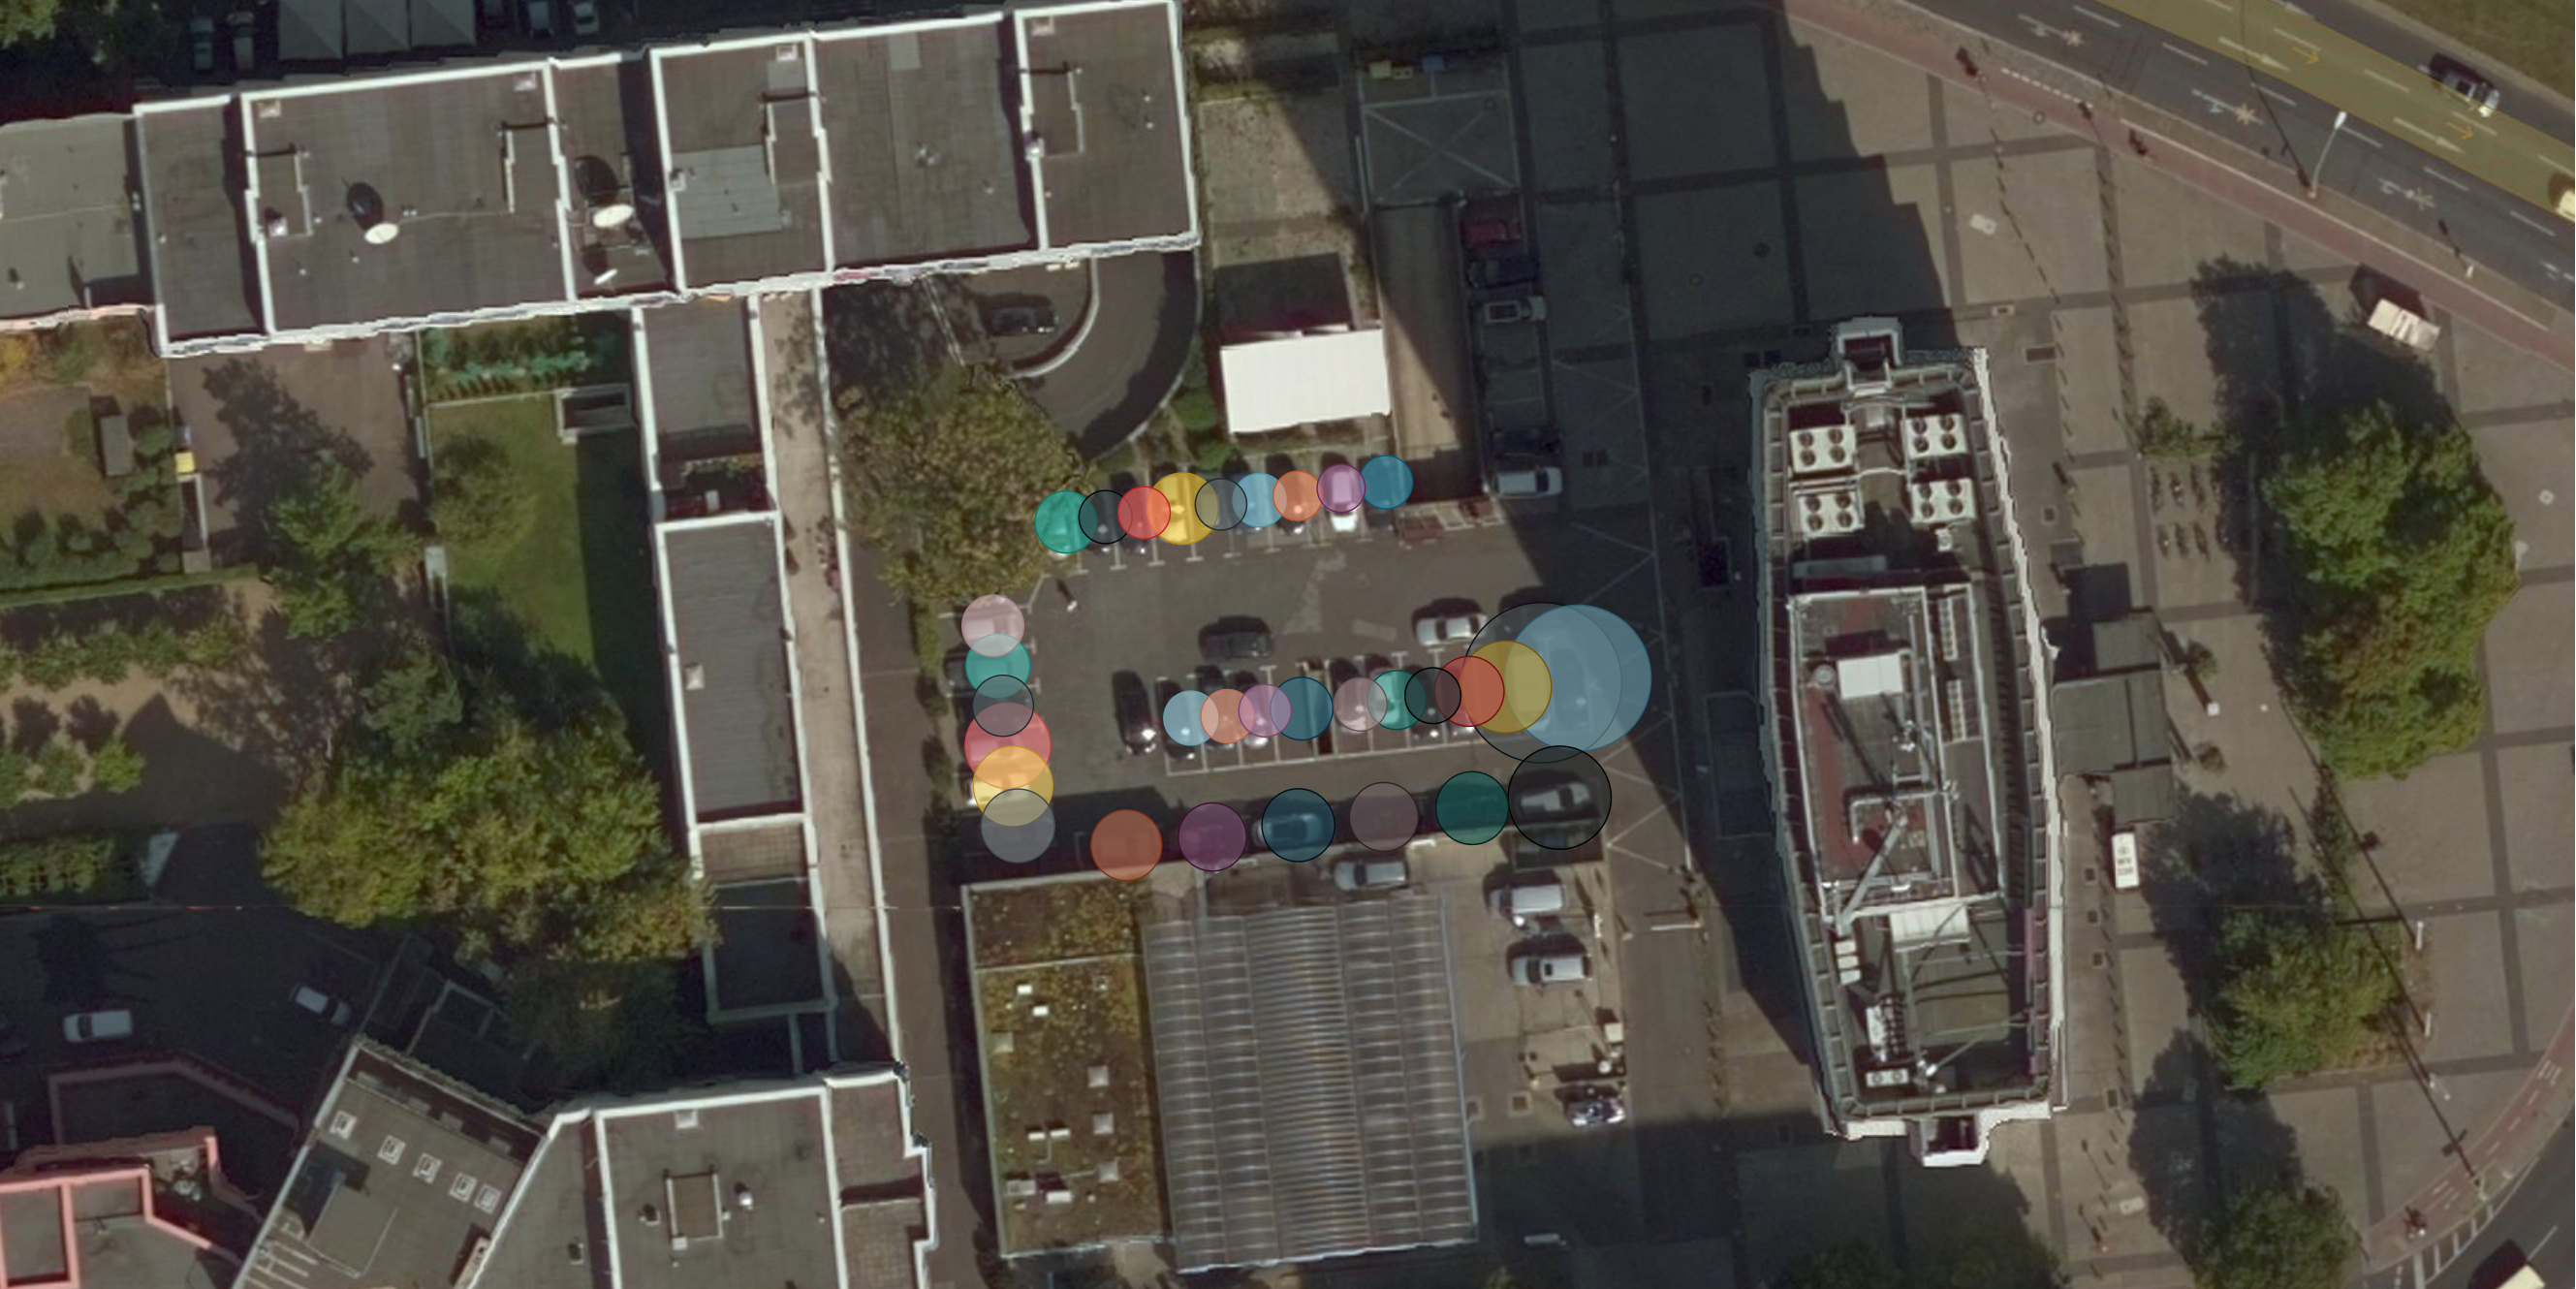
\includegraphics{images/0_parking_map.PNG}
\caption{Sensor\_Locations}
\end{figure}

    \begin{Verbatim}[commandchars=\\\{\}]
{\color{incolor}In [{\color{incolor}7}]:} \PY{n}{parking}\PY{p}{[}\PY{l+s+s1}{\PYZsq{}}\PY{l+s+s1}{Time}\PY{l+s+s1}{\PYZsq{}}\PY{p}{]} \PY{o}{=} \PY{n}{pd}\PY{o}{.}\PY{n}{to\PYZus{}datetime}\PY{p}{(}\PY{n}{parking}\PY{p}{[}\PY{l+s+s1}{\PYZsq{}}\PY{l+s+s1}{Timestamp}\PY{l+s+s1}{\PYZsq{}}\PY{p}{]}\PY{p}{,} \PY{n}{unit}\PY{o}{=}\PY{l+s+s1}{\PYZsq{}}\PY{l+s+s1}{ms}\PY{l+s+s1}{\PYZsq{}}\PY{p}{)}
        \PY{n}{parking}\PY{p}{[}\PY{l+s+s1}{\PYZsq{}}\PY{l+s+s1}{Weekday}\PY{l+s+s1}{\PYZsq{}}\PY{p}{]} \PY{o}{=} \PY{n}{parking}\PY{p}{[}\PY{l+s+s1}{\PYZsq{}}\PY{l+s+s1}{Time}\PY{l+s+s1}{\PYZsq{}}\PY{p}{]}\PY{o}{.}\PY{n}{dt}\PY{o}{.}\PY{n}{dayofweek}
        \PY{n}{parking}\PY{p}{[}\PY{l+s+s1}{\PYZsq{}}\PY{l+s+s1}{Hour}\PY{l+s+s1}{\PYZsq{}}\PY{p}{]} \PY{o}{=} \PY{n}{parking}\PY{p}{[}\PY{l+s+s1}{\PYZsq{}}\PY{l+s+s1}{Time}\PY{l+s+s1}{\PYZsq{}}\PY{p}{]}\PY{o}{.}\PY{n}{dt}\PY{o}{.}\PY{n}{hour}
        \PY{n}{parking} \PY{o}{=} \PY{n}{parking}\PY{o}{.}\PY{n}{sort\PYZus{}values}\PY{p}{(}\PY{n}{by}\PY{o}{=}\PY{p}{[}\PY{l+s+s1}{\PYZsq{}}\PY{l+s+s1}{Timestamp}\PY{l+s+s1}{\PYZsq{}}\PY{p}{]}\PY{p}{)}
        
        \PY{n}{mon} \PY{o}{=} \PY{l+m+mi}{0}
        \PY{n}{tue} \PY{o}{=} \PY{l+m+mi}{0}
        \PY{n}{wed} \PY{o}{=} \PY{l+m+mi}{0}
        \PY{n}{thu} \PY{o}{=} \PY{l+m+mi}{0}
        \PY{n}{fri} \PY{o}{=} \PY{l+m+mi}{0}
        \PY{n}{sat} \PY{o}{=} \PY{l+m+mi}{0}
        \PY{n}{sun} \PY{o}{=} \PY{l+m+mi}{0}
        
        \PY{k}{def} \PY{n+nf}{weekday\PYZus{}parking}\PY{p}{(}\PY{n}{weekday}\PY{p}{,} \PY{n}{fromTime}\PY{p}{,} \PY{n}{toTime}\PY{p}{)}\PY{p}{:}
            \PY{k}{if} \PY{n}{weekday} \PY{o}{!=} \PY{o}{\PYZhy{}}\PY{l+m+mi}{1}\PY{p}{:}
                \PY{n}{day\PYZus{}parking} \PY{o}{=} \PY{n}{parking}\PY{p}{[}\PY{n}{parking}\PY{p}{[}\PY{l+s+s1}{\PYZsq{}}\PY{l+s+s1}{Weekday}\PY{l+s+s1}{\PYZsq{}}\PY{p}{]} \PY{o}{==} \PY{n}{weekday}\PY{p}{]}
            \PY{k}{else}\PY{p}{:}
                \PY{n}{day\PYZus{}parking} \PY{o}{=} \PY{n}{parking}\PY{o}{.}\PY{n}{copy}\PY{p}{(}\PY{p}{)}
                
            \PY{n}{day\PYZus{}parking} \PY{o}{=} \PY{n}{day\PYZus{}parking}\PY{p}{[}\PY{n}{day\PYZus{}parking}\PY{p}{[}\PY{l+s+s1}{\PYZsq{}}\PY{l+s+s1}{Hour}\PY{l+s+s1}{\PYZsq{}}\PY{p}{]} \PY{o}{\PYZgt{}}\PY{o}{=} \PY{n}{fromTime}\PY{p}{]}
            \PY{n}{day\PYZus{}parking} \PY{o}{=} \PY{n}{day\PYZus{}parking}\PY{p}{[}\PY{n}{day\PYZus{}parking}\PY{p}{[}\PY{l+s+s1}{\PYZsq{}}\PY{l+s+s1}{Hour}\PY{l+s+s1}{\PYZsq{}}\PY{p}{]} \PY{o}{\PYZlt{}}\PY{o}{=} \PY{n}{toTime}\PY{p}{]}
        
            \PY{n}{start} \PY{o}{=} \PY{n+nb}{float}\PY{p}{(}\PY{n}{day\PYZus{}parking}\PY{p}{[}\PY{p}{[}\PY{l+s+s1}{\PYZsq{}}\PY{l+s+s1}{Timestamp}\PY{l+s+s1}{\PYZsq{}}\PY{p}{]}\PY{p}{]}\PY{o}{.}\PY{n}{iloc}\PY{p}{[}\PY{l+m+mi}{0}\PY{p}{]}\PY{p}{)}
            \PY{n}{end} \PY{o}{=} \PY{n+nb}{float}\PY{p}{(}\PY{n}{day\PYZus{}parking}\PY{p}{[}\PY{p}{[}\PY{l+s+s1}{\PYZsq{}}\PY{l+s+s1}{Timestamp}\PY{l+s+s1}{\PYZsq{}}\PY{p}{]}\PY{p}{]}\PY{o}{.}\PY{n}{iloc}\PY{p}{[}\PY{o}{\PYZhy{}}\PY{l+m+mi}{1}\PY{p}{]}\PY{p}{)}
            \PY{n}{startDayTime} \PY{o}{=} \PY{n}{day\PYZus{}parking}\PY{p}{[}\PY{p}{[}\PY{l+s+s1}{\PYZsq{}}\PY{l+s+s1}{Time}\PY{l+s+s1}{\PYZsq{}}\PY{p}{]}\PY{p}{]}\PY{o}{.}\PY{n}{iloc}\PY{p}{[}\PY{l+m+mi}{0}\PY{p}{]}\PY{o}{.}\PY{n}{dt}
            \PY{n}{endDayTime} \PY{o}{=} \PY{n}{day\PYZus{}parking}\PY{p}{[}\PY{p}{[}\PY{l+s+s1}{\PYZsq{}}\PY{l+s+s1}{Time}\PY{l+s+s1}{\PYZsq{}}\PY{p}{]}\PY{p}{]}\PY{o}{.}\PY{n}{iloc}\PY{p}{[}\PY{o}{\PYZhy{}}\PY{l+m+mi}{1}\PY{p}{]}\PY{o}{.}\PY{n}{dt}
            
            \PY{n}{lastTime} \PY{o}{=} \PY{n}{startDayTime}
            
            \PY{n}{totalDays} \PY{o}{=} \PY{l+m+mi}{1}
        
            \PY{k}{for} \PY{n}{index}\PY{p}{,} \PY{n}{row} \PY{o+ow}{in} \PY{n}{day\PYZus{}parking}\PY{o}{.}\PY{n}{iterrows}\PY{p}{(}\PY{p}{)}\PY{p}{:}
                \PY{k}{if} \PY{p}{(}\PY{n+nb}{int}\PY{p}{(}\PY{n}{row}\PY{p}{[}\PY{l+s+s1}{\PYZsq{}}\PY{l+s+s1}{Time}\PY{l+s+s1}{\PYZsq{}}\PY{p}{]}\PY{o}{.}\PY{n}{day}\PY{p}{)} \PY{o}{!=} \PY{n+nb}{int}\PY{p}{(}\PY{n}{lastTime}\PY{o}{.}\PY{n}{day}\PY{p}{)}\PY{p}{)}\PY{p}{:}
                    \PY{n}{lastTime} \PY{o}{=} \PY{n}{row}\PY{p}{[}\PY{l+s+s1}{\PYZsq{}}\PY{l+s+s1}{Time}\PY{l+s+s1}{\PYZsq{}}\PY{p}{]}
                    \PY{n}{totalDays}\PY{o}{+}\PY{o}{=}\PY{l+m+mi}{1}
                    
        
            \PY{n}{totalTime} \PY{o}{=} \PY{n}{timedelta}\PY{p}{(}\PY{n}{days}\PY{o}{=}\PY{n}{totalDays}\PY{p}{)}
            \PY{n}{totalTime} \PY{o}{\PYZhy{}}\PY{o}{=} \PY{n}{timedelta}\PY{p}{(}\PY{n}{hours}\PY{o}{=}\PY{n+nb}{int}\PY{p}{(}\PY{n}{startDayTime}\PY{o}{.}\PY{n}{hour}\PY{p}{)}\PY{p}{)}
            \PY{n}{totalTime} \PY{o}{\PYZhy{}}\PY{o}{=} \PY{n}{timedelta}\PY{p}{(}\PY{n}{hours}\PY{o}{=}\PY{p}{(}\PY{l+m+mi}{24} \PY{o}{\PYZhy{}} \PY{n+nb}{int}\PY{p}{(}\PY{n}{endDayTime}\PY{o}{.}\PY{n}{hour}\PY{p}{)}\PY{p}{)}\PY{p}{)}
            \PY{n}{totalTime} \PY{o}{\PYZhy{}}\PY{o}{=} \PY{n}{timedelta}\PY{p}{(}\PY{n}{hours}\PY{o}{=}\PY{n}{totalDays}\PY{o}{*}\PY{n}{fromTime}\PY{p}{)}
            \PY{n}{totalTime} \PY{o}{\PYZhy{}}\PY{o}{=} \PY{n}{timedelta}\PY{p}{(}\PY{n}{hours}\PY{o}{=}\PY{n}{totalDays}\PY{o}{*}\PY{p}{(}\PY{l+m+mi}{24}\PY{o}{\PYZhy{}}\PY{n}{toTime}\PY{p}{)}\PY{p}{)}
            
            \PY{n}{mean\PYZus{}weekday\PYZus{}parking} \PY{o}{=} \PY{p}{\PYZob{}}\PY{p}{\PYZcb{}}
            
            \PY{k}{for} \PY{n}{key} \PY{o+ow}{in} \PY{n}{parking\PYZus{}latlon}\PY{p}{:}
                \PY{n}{temp} \PY{o}{=} \PY{n}{day\PYZus{}parking}\PY{p}{[}\PY{n}{day\PYZus{}parking}\PY{p}{[}\PY{l+s+s1}{\PYZsq{}}\PY{l+s+s1}{ParkingSpotID}\PY{l+s+s1}{\PYZsq{}}\PY{p}{]} \PY{o}{==} \PY{n}{key}\PY{p}{]}\PY{p}{[}\PY{p}{[}\PY{l+s+s1}{\PYZsq{}}\PY{l+s+s1}{Timestamp}\PY{l+s+s1}{\PYZsq{}}\PY{p}{,}\PY{l+s+s1}{\PYZsq{}}\PY{l+s+s1}{Occupied}\PY{l+s+s1}{\PYZsq{}}\PY{p}{,}\PY{l+s+s1}{\PYZsq{}}\PY{l+s+s1}{Time}\PY{l+s+s1}{\PYZsq{}}\PY{p}{]}\PY{p}{]}
                \PY{k}{if} \PY{n+nb}{len}\PY{p}{(}\PY{n}{temp}\PY{p}{)} \PY{o}{\PYZgt{}} \PY{l+m+mi}{0}\PY{p}{:}
                    \PY{n}{occupied} \PY{o}{=} \PY{n}{temp}\PY{o}{.}\PY{n}{iloc}\PY{p}{[}\PY{l+m+mi}{0}\PY{p}{]}\PY{p}{[}\PY{l+s+s1}{\PYZsq{}}\PY{l+s+s1}{Occupied}\PY{l+s+s1}{\PYZsq{}}\PY{p}{]} \PY{o}{==} \PY{l+m+mi}{1}
                    \PY{n}{lastTime} \PY{o}{=} \PY{n}{start}
                    \PY{n}{lastDayTime} \PY{o}{=} \PY{n}{startDayTime}
                    \PY{n}{mean\PYZus{}weekday\PYZus{}parking}\PY{p}{[}\PY{n}{key}\PY{p}{]} \PY{o}{=} \PY{l+m+mi}{0}
        
                    \PY{k}{for} \PY{n}{index}\PY{p}{,} \PY{n}{row} \PY{o+ow}{in} \PY{n}{temp}\PY{o}{.}\PY{n}{iterrows}\PY{p}{(}\PY{p}{)}\PY{p}{:}
                        \PY{c+c1}{\PYZsh{}\PYZsh{}cut off when the day switches}
                        \PY{k}{if} \PY{p}{(}\PY{n+nb}{int}\PY{p}{(}\PY{n}{row}\PY{p}{[}\PY{l+s+s1}{\PYZsq{}}\PY{l+s+s1}{Time}\PY{l+s+s1}{\PYZsq{}}\PY{p}{]}\PY{o}{.}\PY{n}{day}\PY{p}{)} \PY{o}{!=} \PY{n+nb}{int}\PY{p}{(}\PY{n}{lastDayTime}\PY{o}{.}\PY{n}{day}\PY{p}{)}\PY{p}{)}\PY{p}{:}
                            \PY{k}{if} \PY{n}{occupied}\PY{p}{:}
                                \PY{c+c1}{\PYZsh{}\PYZsh{}add time till the end of the day}
                                \PY{n}{endOfDay} \PY{o}{=} \PY{n}{timedelta}\PY{p}{(}\PY{n}{hours}\PY{o}{=}\PY{p}{(}\PY{l+m+mi}{24}\PY{o}{\PYZhy{}}\PY{n+nb}{int}\PY{p}{(}\PY{n}{lastDayTime}\PY{o}{.}\PY{n}{hour}\PY{p}{)}\PY{p}{)}\PY{p}{)}
                                \PY{n}{mean\PYZus{}weekday\PYZus{}parking}\PY{p}{[}\PY{n}{key}\PY{p}{]} \PY{o}{+}\PY{o}{=} \PY{p}{(}\PY{n}{endOfDay}\PY{o}{.}\PY{n}{total\PYZus{}seconds}\PY{p}{(}\PY{p}{)} \PY{o}{*} \PY{l+m+mi}{1000}\PY{p}{)}
        
                            \PY{n}{lastTime} \PY{o}{=} \PY{n}{row}\PY{p}{[}\PY{l+s+s1}{\PYZsq{}}\PY{l+s+s1}{Timestamp}\PY{l+s+s1}{\PYZsq{}}\PY{p}{]}
                            \PY{n}{lastDayTime} \PY{o}{=} \PY{n}{row}\PY{p}{[}\PY{l+s+s1}{\PYZsq{}}\PY{l+s+s1}{Time}\PY{l+s+s1}{\PYZsq{}}\PY{p}{]}
                            \PY{n}{occupied} \PY{o}{=} \PY{n}{row}\PY{p}{[}\PY{l+s+s1}{\PYZsq{}}\PY{l+s+s1}{Occupied}\PY{l+s+s1}{\PYZsq{}}\PY{p}{]} \PY{o}{==} \PY{l+m+mi}{1}
                        \PY{k}{else}\PY{p}{:}
                            \PY{k}{if} \PY{n}{occupied} \PY{o}{!=} \PY{p}{(}\PY{n}{row}\PY{p}{[}\PY{l+s+s1}{\PYZsq{}}\PY{l+s+s1}{Occupied}\PY{l+s+s1}{\PYZsq{}}\PY{p}{]} \PY{o}{==} \PY{l+m+mi}{1}\PY{p}{)}\PY{p}{:}
                                \PY{k}{if} \PY{n}{occupied}\PY{p}{:}
                                    \PY{n}{mean\PYZus{}weekday\PYZus{}parking}\PY{p}{[}\PY{n}{key}\PY{p}{]} \PY{o}{+}\PY{o}{=} \PY{n}{row}\PY{p}{[}\PY{l+s+s1}{\PYZsq{}}\PY{l+s+s1}{Timestamp}\PY{l+s+s1}{\PYZsq{}}\PY{p}{]} \PY{o}{\PYZhy{}} \PY{n}{lastTime}
                                \PY{k}{else}\PY{p}{:}
                                    \PY{n}{lastTime} \PY{o}{=} \PY{n}{row}\PY{p}{[}\PY{l+s+s1}{\PYZsq{}}\PY{l+s+s1}{Timestamp}\PY{l+s+s1}{\PYZsq{}}\PY{p}{]}
                                \PY{n}{occupied} \PY{o}{=} \PY{n}{row}\PY{p}{[}\PY{l+s+s1}{\PYZsq{}}\PY{l+s+s1}{Occupied}\PY{l+s+s1}{\PYZsq{}}\PY{p}{]} \PY{o}{==} \PY{l+m+mi}{1}
        
                    \PY{k}{if} \PY{n}{occupied}\PY{p}{:}
                        \PY{n}{mean\PYZus{}weekday\PYZus{}parking}\PY{p}{[}\PY{n}{key}\PY{p}{]} \PY{o}{+}\PY{o}{=} \PY{n}{end} \PY{o}{\PYZhy{}} \PY{n}{lastTime}
        
                    \PY{n}{mean\PYZus{}weekday\PYZus{}parking}\PY{p}{[}\PY{n}{key}\PY{p}{]} \PY{o}{/}\PY{o}{=} \PY{p}{(}\PY{n}{totalTime}\PY{o}{.}\PY{n}{total\PYZus{}seconds}\PY{p}{(}\PY{p}{)} \PY{o}{*} \PY{l+m+mi}{1000}\PY{p}{)}
                    
                    \PY{k}{if} \PY{n}{mean\PYZus{}weekday\PYZus{}parking}\PY{p}{[}\PY{n}{key}\PY{p}{]} \PY{o}{\PYZgt{}} \PY{l+m+mi}{1}\PY{p}{:}
                        \PY{n}{mean\PYZus{}weekday\PYZus{}parking}\PY{p}{[}\PY{n}{key}\PY{p}{]} \PY{o}{=} \PY{l+m+mi}{1}
                    \PY{c+c1}{\PYZsh{}\PYZsh{}print(key, \PYZdq{}:\PYZdq{}, mean\PYZus{}weekday\PYZus{}parking[key])}
            
            \PY{k}{return} \PY{n}{mean\PYZus{}weekday\PYZus{}parking}\PY{p}{;}
        
        
        \PY{k}{def} \PY{n+nf}{show\PYZus{}parking}\PY{p}{(}\PY{n}{data}\PY{p}{)}\PY{p}{:}
            \PY{n}{parkplatz\PYZus{}center} \PY{o}{=} \PY{p}{[}\PY{l+m+mf}{52.513025}\PY{p}{,} \PY{l+m+mf}{13.319505}\PY{p}{]}
            \PY{n}{parking\PYZus{}map} \PY{o}{=} \PY{n}{folium}\PY{o}{.}\PY{n}{Map}\PY{p}{(}\PY{n}{location}\PY{o}{=}\PY{n}{parkplatz\PYZus{}center}\PY{p}{,} \PY{n}{zoom\PYZus{}start}\PY{o}{=}\PY{l+m+mi}{18}\PY{p}{)}
        
            \PY{k}{for} \PY{n}{key} \PY{o+ow}{in} \PY{n}{parking\PYZus{}latlon}\PY{p}{:}
                \PY{k}{if} \PY{n}{key} \PY{o+ow}{in} \PY{n}{data}\PY{p}{:}
                    \PY{n}{visual} \PY{o}{=} \PY{n}{data}\PY{p}{[}\PY{n}{key}\PY{p}{]}
                    \PY{n}{folium}\PY{o}{.}\PY{n}{Circle}\PY{p}{(}
                        \PY{n}{radius}\PY{o}{=}\PY{l+m+mi}{1}\PY{p}{,}
                        \PY{n}{location}\PY{o}{=}\PY{n}{parking\PYZus{}latlon}\PY{p}{[}\PY{n}{key}\PY{p}{]}\PY{p}{,}
                        \PY{n}{popup}\PY{o}{=}\PY{n}{key} \PY{o}{+} \PY{l+s+s2}{\PYZdq{}}\PY{l+s+s2}{: }\PY{l+s+s2}{\PYZdq{}} \PY{o}{+} \PY{n+nb}{str}\PY{p}{(}\PY{n+nb}{int}\PY{p}{(}\PY{n}{visual}\PY{o}{*}\PY{l+m+mi}{100}\PY{p}{)}\PY{p}{)} \PY{o}{+} \PY{l+s+s2}{\PYZdq{}}\PY{l+s+s2}{\PYZpc{}}\PY{l+s+s2}{\PYZdq{}}\PY{p}{,}
                        \PY{n}{color}\PY{o}{=}\PY{l+s+s1}{\PYZsq{}}\PY{l+s+s1}{\PYZsh{}}\PY{l+s+si}{\PYZpc{}02x}\PY{l+s+si}{\PYZpc{}02x}\PY{l+s+si}{\PYZpc{}02x}\PY{l+s+s1}{\PYZsq{}} \PY{o}{\PYZpc{}} \PY{p}{(}\PY{n+nb}{int}\PY{p}{(}\PY{l+m+mi}{255} \PY{o}{*} \PY{p}{(}\PY{l+m+mi}{1}\PY{o}{\PYZhy{}}\PY{n}{visual}\PY{p}{)}\PY{p}{)}\PY{p}{,}\PY{n+nb}{int}\PY{p}{(}\PY{l+m+mi}{255} \PY{o}{*} \PY{p}{(}\PY{l+m+mi}{1}\PY{o}{\PYZhy{}}\PY{n}{visual}\PY{p}{)}\PY{p}{)}\PY{p}{,} \PY{n+nb}{int}\PY{p}{(}\PY{l+m+mi}{255} \PY{o}{*} \PY{p}{(}\PY{l+m+mi}{1}\PY{o}{\PYZhy{}}\PY{n}{visual}\PY{p}{)}\PY{p}{)}\PY{p}{)}\PY{p}{,}
                        \PY{n}{fill}\PY{o}{=}\PY{k+kc}{True}
                    \PY{p}{)}\PY{o}{.}\PY{n}{add\PYZus{}to}\PY{p}{(}\PY{n}{parking\PYZus{}map}\PY{p}{)}
            \PY{k}{return} \PY{n}{parking\PYZus{}map}\PY{p}{;}
         
        
        \PY{c+c1}{\PYZsh{}\PYZsh{} schwarz = häufig belegt, weiß = weniger häufig belegt}
        \PY{c+c1}{\PYZsh{} TODO: Prozente }
        \PY{n}{show\PYZus{}parking}\PY{p}{(}\PY{n}{weekday\PYZus{}parking}\PY{p}{(}\PY{o}{\PYZhy{}}\PY{l+m+mi}{1}\PY{p}{,} \PY{l+m+mi}{6}\PY{p}{,} \PY{l+m+mi}{22}\PY{p}{)}\PY{p}{)}
\end{Verbatim}


\begin{Verbatim}[commandchars=\\\{\}]
{\color{outcolor}Out[{\color{outcolor}7}]:} <folium.folium.Map at 0x1a154ac400>
\end{Verbatim}
            
    \begin{Verbatim}[commandchars=\\\{\}]
{\color{incolor}In [{\color{incolor}8}]:} \PY{n}{show\PYZus{}parking}\PY{p}{(}\PY{n}{weekday\PYZus{}parking}\PY{p}{(}\PY{l+m+mi}{3}\PY{p}{,} \PY{l+m+mi}{6}\PY{p}{,} \PY{l+m+mi}{22}\PY{p}{)}\PY{p}{)}
\end{Verbatim}


\begin{Verbatim}[commandchars=\\\{\}]
{\color{outcolor}Out[{\color{outcolor}8}]:} <folium.folium.Map at 0x1a154d3550>
\end{Verbatim}
            
    \begin{Verbatim}[commandchars=\\\{\}]
{\color{incolor}In [{\color{incolor}9}]:} \PY{n}{show\PYZus{}parking}\PY{p}{(}\PY{n}{weekday\PYZus{}parking}\PY{p}{(}\PY{l+m+mi}{6}\PY{p}{,} \PY{l+m+mi}{6}\PY{p}{,} \PY{l+m+mi}{22}\PY{p}{)}\PY{p}{)}
\end{Verbatim}


\begin{Verbatim}[commandchars=\\\{\}]
{\color{outcolor}Out[{\color{outcolor}9}]:} <folium.folium.Map at 0x1a15607208>
\end{Verbatim}
            
    \begin{Verbatim}[commandchars=\\\{\}]
{\color{incolor}In [{\color{incolor}10}]:} \PY{n}{show\PYZus{}parking}\PY{p}{(}\PY{n}{weekday\PYZus{}parking}\PY{p}{(}\PY{o}{\PYZhy{}}\PY{l+m+mi}{1}\PY{p}{,} \PY{l+m+mi}{6}\PY{p}{,} \PY{l+m+mi}{14}\PY{p}{)}\PY{p}{)}
\end{Verbatim}


\begin{Verbatim}[commandchars=\\\{\}]
{\color{outcolor}Out[{\color{outcolor}10}]:} <folium.folium.Map at 0x1a1567ae10>
\end{Verbatim}
            
    \begin{Verbatim}[commandchars=\\\{\}]
{\color{incolor}In [{\color{incolor}11}]:} \PY{n}{show\PYZus{}parking}\PY{p}{(}\PY{n}{weekday\PYZus{}parking}\PY{p}{(}\PY{o}{\PYZhy{}}\PY{l+m+mi}{1}\PY{p}{,} \PY{l+m+mi}{14}\PY{p}{,} \PY{l+m+mi}{22}\PY{p}{)}\PY{p}{)}
\end{Verbatim}


\begin{Verbatim}[commandchars=\\\{\}]
{\color{outcolor}Out[{\color{outcolor}11}]:} <folium.folium.Map at 0x1a15727b38>
\end{Verbatim}
            
    \begin{figure}
\centering
\includegraphics{images/1_parking_average.PNG}
\caption{Parking\_Average}
\end{figure}

    \begin{figure}
\centering
\includegraphics{images/2_parking_daytime.PNG}
\caption{Parking\_Daytime}
\end{figure}

    \begin{figure}
\centering
\includegraphics{images/3_parking_weekdays.PNG}
\caption{Parking\_Weekdays}
\end{figure}

    \begin{figure}
\centering
\includegraphics{images/4_parking_weekdays_ranked.PNG}
\caption{Parking\_Weekdays}
\end{figure}

    \begin{figure}
\centering
\includegraphics{images/5_parking_weekdays_frequency_ranked.PNG}
\caption{Parking\_Frequency}
\end{figure}

    \begin{figure}
\centering
\includegraphics{images/6_parking_top5.PNG}
\caption{Parking\_Top5}
\end{figure}

    \begin{figure}
\centering
\includegraphics{images/7_parking_top5_daytime.PNG}
\caption{Parking\_Top5\_Daytime}
\end{figure}

    \begin{figure}
\centering
\includegraphics{images/_powerBI_slides/01_parking.PNG}
\caption{Parking\_PBI\_1}
\end{figure}

    \begin{figure}
\centering
\includegraphics{images/_powerBI_slides/02_parking.PNG}
\caption{Parking\_PBI\_2}
\end{figure}

    \begin{figure}
\centering
\includegraphics{images/_powerBI_slides/03_parkingMap.PNG}
\caption{Parking\_PBI\_3}
\end{figure}

    \section{Traffic}\label{traffic}

\begin{figure}
\centering
\includegraphics{images/_powerBI_slides/carCountSensorsMap.PNG}
\caption{Sensor\_Locations}
\end{figure}

    \begin{figure}
\centering
\includegraphics{images/_powerBI_slides/averageCarCountCalendar.PNG}
\caption{Traffic\_PBI\_1}
\end{figure}

    \begin{figure}
\centering
\includegraphics{images/_powerBI_slides/averageCountCarSensorCalendar.PNG}
\caption{Traffic\_PBI\_2}
\end{figure}

    \begin{figure}
\centering
\includegraphics{images/_powerBI_slides/highDensityCarType.PNG}
\caption{Traffic\_PBI\_3}
\end{figure}

    \begin{figure}
\centering
\includegraphics{images/_powerBI_slides/04_traffic.PNG}
\caption{Traffic\_PBI\_4}
\end{figure}

    \subsection{Pedestrians}\label{pedestrians}

    \begin{Verbatim}[commandchars=\\\{\}]
{\color{incolor}In [{\color{incolor}12}]:} \PY{o}{\PYZpc{}}\PY{k}{pylab} inline
         \PY{n}{pylab}\PY{o}{.}\PY{n}{rcParams}\PY{p}{[}\PY{l+s+s1}{\PYZsq{}}\PY{l+s+s1}{figure.figsize}\PY{l+s+s1}{\PYZsq{}}\PY{p}{]} \PY{o}{=} \PY{p}{(}\PY{l+m+mi}{15}\PY{p}{,} \PY{l+m+mi}{10}\PY{p}{)}
         \PY{n}{pylab}\PY{o}{.}\PY{n}{rcParams}\PY{p}{[}\PY{l+s+s1}{\PYZsq{}}\PY{l+s+s1}{figure.dpi}\PY{l+s+s1}{\PYZsq{}}\PY{p}{]} \PY{o}{=} \PY{l+m+mi}{200}
\end{Verbatim}


    \begin{Verbatim}[commandchars=\\\{\}]
Populating the interactive namespace from numpy and matplotlib

    \end{Verbatim}

    \begin{Verbatim}[commandchars=\\\{\}]
{\color{incolor}In [{\color{incolor}13}]:} \PY{n}{df\PYZus{}pedestrians\PYZus{}original} \PY{o}{=} \PY{n}{pd}\PY{o}{.}\PY{n}{read\PYZus{}csv}\PY{p}{(}\PY{l+s+s1}{\PYZsq{}}\PY{l+s+s1}{data/pedestrian\PYZus{}counts\PYZus{}tel\PYZus{}a.csv}\PY{l+s+s1}{\PYZsq{}}\PY{p}{,} \PY{n}{sep}\PY{o}{=}\PY{l+s+s2}{\PYZdq{}}\PY{l+s+s2}{ }\PY{l+s+s2}{\PYZdq{}}\PY{p}{)}
         \PY{n+nb}{print}\PY{p}{(}\PY{l+s+s1}{\PYZsq{}}\PY{l+s+s1}{Total number of entries: }\PY{l+s+se}{\PYZbs{}n}\PY{l+s+se}{\PYZbs{}n}\PY{l+s+s1}{\PYZsq{}} \PY{o}{+} \PY{n+nb}{str}\PY{p}{(}\PY{n}{df\PYZus{}pedestrians\PYZus{}original}\PY{o}{.}\PY{n}{count}\PY{p}{(}\PY{p}{)}\PY{p}{)}\PY{p}{)}
         \PY{n+nb}{print}\PY{p}{(}\PY{l+s+s1}{\PYZsq{}}\PY{l+s+se}{\PYZbs{}n}\PY{l+s+se}{\PYZbs{}n}\PY{l+s+s1}{Example Output: }\PY{l+s+s1}{\PYZsq{}}\PY{p}{)}
         \PY{n}{df\PYZus{}pedestrians\PYZus{}original}\PY{o}{.}\PY{n}{head}\PY{p}{(}\PY{p}{)}
\end{Verbatim}


    \begin{Verbatim}[commandchars=\\\{\}]
Total number of entries: 

StationIdentifier    402616
Timestamp            402616
Direction            402616
Count                402616
dtype: int64


Example Output: 

    \end{Verbatim}

\begin{Verbatim}[commandchars=\\\{\}]
{\color{outcolor}Out[{\color{outcolor}13}]:}                         StationIdentifier      Timestamp Direction  Count
         0    CounterVorplatzGeb-AF2-PeopleCounter  1515525300416        IN      0
         1    CounterVorplatzGeb-AF2-PeopleCounter  1515525300418       OUT      0
         2  CounterHaupteingang-TEL4-PeopleCounter  1515525300417        IN      0
         3  CounterHaupteingang-TEL4-PeopleCounter  1515525300415       OUT      0
         4    CounterVorplatzGeb-AF2-PeopleCounter  1515525360372        IN      0
\end{Verbatim}
            
    \subsubsection{Clean}\label{clean}

    \begin{Verbatim}[commandchars=\\\{\}]
{\color{incolor}In [{\color{incolor}14}]:} \PY{c+c1}{\PYZsh{} clone for backup}
         \PY{n}{df\PYZus{}pedestrians} \PY{o}{=} \PY{n}{df\PYZus{}pedestrians\PYZus{}original}
         \PY{c+c1}{\PYZsh{} rename}
         \PY{n}{df\PYZus{}pedestrians} \PY{o}{=} \PY{n}{df\PYZus{}pedestrians}\PY{o}{.}\PY{n}{replace}\PY{p}{(}\PY{p}{\PYZob{}}\PY{l+s+s1}{\PYZsq{}}\PY{l+s+s1}{CounterVorplatzGeb\PYZhy{}AF2\PYZhy{}PeopleCounter}\PY{l+s+s1}{\PYZsq{}}\PY{p}{:}\PY{l+s+s1}{\PYZsq{}}\PY{l+s+s1}{af\PYZus{}counter}\PY{l+s+s1}{\PYZsq{}}\PY{p}{,} \PY{l+s+s1}{\PYZsq{}}\PY{l+s+s1}{CounterHaupteingang\PYZhy{}TEL4\PYZhy{}PeopleCounter}\PY{l+s+s1}{\PYZsq{}}\PY{p}{:}\PY{l+s+s1}{\PYZsq{}}\PY{l+s+s1}{telekom\PYZus{}counter}\PY{l+s+s1}{\PYZsq{}}\PY{p}{\PYZcb{}}\PY{p}{)}
         \PY{c+c1}{\PYZsh{} drop zero counts}
         \PY{n}{df\PYZus{}pedestrians} \PY{o}{=} \PY{n}{df\PYZus{}pedestrians}\PY{p}{[}\PY{n}{df\PYZus{}pedestrians}\PY{o}{.}\PY{n}{Count} \PY{o}{!=} \PY{l+m+mi}{0}\PY{p}{]}
         \PY{c+c1}{\PYZsh{} timestamp to python data type}
         \PY{n}{df\PYZus{}pedestrians}\PY{p}{[}\PY{l+s+s1}{\PYZsq{}}\PY{l+s+s1}{Timestamp}\PY{l+s+s1}{\PYZsq{}}\PY{p}{]} \PY{o}{=} \PY{n}{pd}\PY{o}{.}\PY{n}{to\PYZus{}datetime}\PY{p}{(}\PY{n}{df\PYZus{}pedestrians}\PY{p}{[}\PY{l+s+s1}{\PYZsq{}}\PY{l+s+s1}{Timestamp}\PY{l+s+s1}{\PYZsq{}}\PY{p}{]}\PY{o}{.}\PY{n}{astype}\PY{p}{(}\PY{n+nb}{int}\PY{p}{)}\PY{p}{,} \PY{n}{unit}\PY{o}{=}\PY{l+s+s1}{\PYZsq{}}\PY{l+s+s1}{ms}\PY{l+s+s1}{\PYZsq{}}\PY{p}{)}
\end{Verbatim}


    \subsubsection{Verify Dataset Integrity}\label{verify-dataset-integrity}

    \begin{Verbatim}[commandchars=\\\{\}]
{\color{incolor}In [{\color{incolor}15}]:} \PY{n}{df\PYZus{}pedestrians\PYZus{}IN} \PY{o}{=} \PY{n}{df\PYZus{}pedestrians}\PY{p}{[}\PY{n}{df\PYZus{}pedestrians}\PY{p}{[}\PY{l+s+s1}{\PYZsq{}}\PY{l+s+s1}{Direction}\PY{l+s+s1}{\PYZsq{}}\PY{p}{]} \PY{o}{==} \PY{l+s+s1}{\PYZsq{}}\PY{l+s+s1}{IN}\PY{l+s+s1}{\PYZsq{}}\PY{p}{]} 
         \PY{n}{df\PYZus{}pedestrians\PYZus{}OUT} \PY{o}{=} \PY{n}{df\PYZus{}pedestrians}\PY{p}{[}\PY{n}{df\PYZus{}pedestrians}\PY{p}{[}\PY{l+s+s1}{\PYZsq{}}\PY{l+s+s1}{Direction}\PY{l+s+s1}{\PYZsq{}}\PY{p}{]} \PY{o}{==} \PY{l+s+s1}{\PYZsq{}}\PY{l+s+s1}{OUT}\PY{l+s+s1}{\PYZsq{}}\PY{p}{]}
\end{Verbatim}


    \begin{Verbatim}[commandchars=\\\{\}]
{\color{incolor}In [{\color{incolor}16}]:} \PY{n}{df\PYZus{}pedestrians\PYZus{}IN\PYZus{}af} \PY{o}{=} \PY{n}{df\PYZus{}pedestrians\PYZus{}IN}\PY{p}{[}\PY{n}{df\PYZus{}pedestrians\PYZus{}IN}\PY{p}{[}\PY{l+s+s1}{\PYZsq{}}\PY{l+s+s1}{StationIdentifier}\PY{l+s+s1}{\PYZsq{}}\PY{p}{]} \PY{o}{==} \PY{l+s+s1}{\PYZsq{}}\PY{l+s+s1}{af\PYZus{}counter}\PY{l+s+s1}{\PYZsq{}}\PY{p}{]}
         \PY{n}{df\PYZus{}pedestrians\PYZus{}OUT\PYZus{}af} \PY{o}{=} \PY{n}{df\PYZus{}pedestrians\PYZus{}OUT}\PY{p}{[}\PY{n}{df\PYZus{}pedestrians\PYZus{}OUT}\PY{p}{[}\PY{l+s+s1}{\PYZsq{}}\PY{l+s+s1}{StationIdentifier}\PY{l+s+s1}{\PYZsq{}}\PY{p}{]} \PY{o}{==} \PY{l+s+s1}{\PYZsq{}}\PY{l+s+s1}{af\PYZus{}counter}\PY{l+s+s1}{\PYZsq{}}\PY{p}{]}
         \PY{n}{df\PYZus{}pedestrians\PYZus{}IN\PYZus{}tel} \PY{o}{=} \PY{n}{df\PYZus{}pedestrians\PYZus{}IN}\PY{p}{[}\PY{n}{df\PYZus{}pedestrians\PYZus{}IN}\PY{p}{[}\PY{l+s+s1}{\PYZsq{}}\PY{l+s+s1}{StationIdentifier}\PY{l+s+s1}{\PYZsq{}}\PY{p}{]} \PY{o}{==} \PY{l+s+s1}{\PYZsq{}}\PY{l+s+s1}{telekom\PYZus{}counter}\PY{l+s+s1}{\PYZsq{}}\PY{p}{]}
         \PY{n}{df\PYZus{}pedestrians\PYZus{}OUT\PYZus{}tel} \PY{o}{=} \PY{n}{df\PYZus{}pedestrians\PYZus{}OUT}\PY{p}{[}\PY{n}{df\PYZus{}pedestrians\PYZus{}OUT}\PY{p}{[}\PY{l+s+s1}{\PYZsq{}}\PY{l+s+s1}{StationIdentifier}\PY{l+s+s1}{\PYZsq{}}\PY{p}{]} \PY{o}{==} \PY{l+s+s1}{\PYZsq{}}\PY{l+s+s1}{telekom\PYZus{}counter}\PY{l+s+s1}{\PYZsq{}}\PY{p}{]}
         
         \PY{n}{count\PYZus{}total\PYZus{}IN\PYZus{}records} \PY{o}{=} \PY{n}{df\PYZus{}pedestrians\PYZus{}IN}\PY{p}{[}\PY{l+s+s1}{\PYZsq{}}\PY{l+s+s1}{Count}\PY{l+s+s1}{\PYZsq{}}\PY{p}{]}\PY{o}{.}\PY{n}{count}\PY{p}{(}\PY{p}{)}
         \PY{n}{count\PYZus{}total\PYZus{}OUT\PYZus{}records} \PY{o}{=} \PY{n}{df\PYZus{}pedestrians\PYZus{}OUT}\PY{p}{[}\PY{l+s+s1}{\PYZsq{}}\PY{l+s+s1}{Count}\PY{l+s+s1}{\PYZsq{}}\PY{p}{]}\PY{o}{.}\PY{n}{count}\PY{p}{(}\PY{p}{)}
         \PY{n}{count\PYZus{}walked\PYZus{}IN\PYZus{}af} \PY{o}{=} \PY{n}{df\PYZus{}pedestrians\PYZus{}IN\PYZus{}af}\PY{o}{.}\PY{n}{Count}\PY{o}{.}\PY{n}{sum}\PY{p}{(}\PY{p}{)}
         \PY{n}{count\PYZus{}walked\PYZus{}OUT\PYZus{}af} \PY{o}{=} \PY{n}{df\PYZus{}pedestrians\PYZus{}OUT\PYZus{}af}\PY{o}{.}\PY{n}{Count}\PY{o}{.}\PY{n}{sum}\PY{p}{(}\PY{p}{)}
         \PY{n}{count\PYZus{}walked\PYZus{}IN\PYZus{}tel} \PY{o}{=} \PY{n}{df\PYZus{}pedestrians\PYZus{}IN\PYZus{}tel}\PY{o}{.}\PY{n}{Count}\PY{o}{.}\PY{n}{sum}\PY{p}{(}\PY{p}{)}
         \PY{n}{count\PYZus{}walked\PYZus{}OUT\PYZus{}tel} \PY{o}{=} \PY{n}{df\PYZus{}pedestrians\PYZus{}OUT\PYZus{}tel}\PY{o}{.}\PY{n}{Count}\PY{o}{.}\PY{n}{sum}\PY{p}{(}\PY{p}{)}
\end{Verbatim}


    \subsubsection{Fußgänger}\label{fuuxdfguxe4nger}

\begin{figure}
\centering
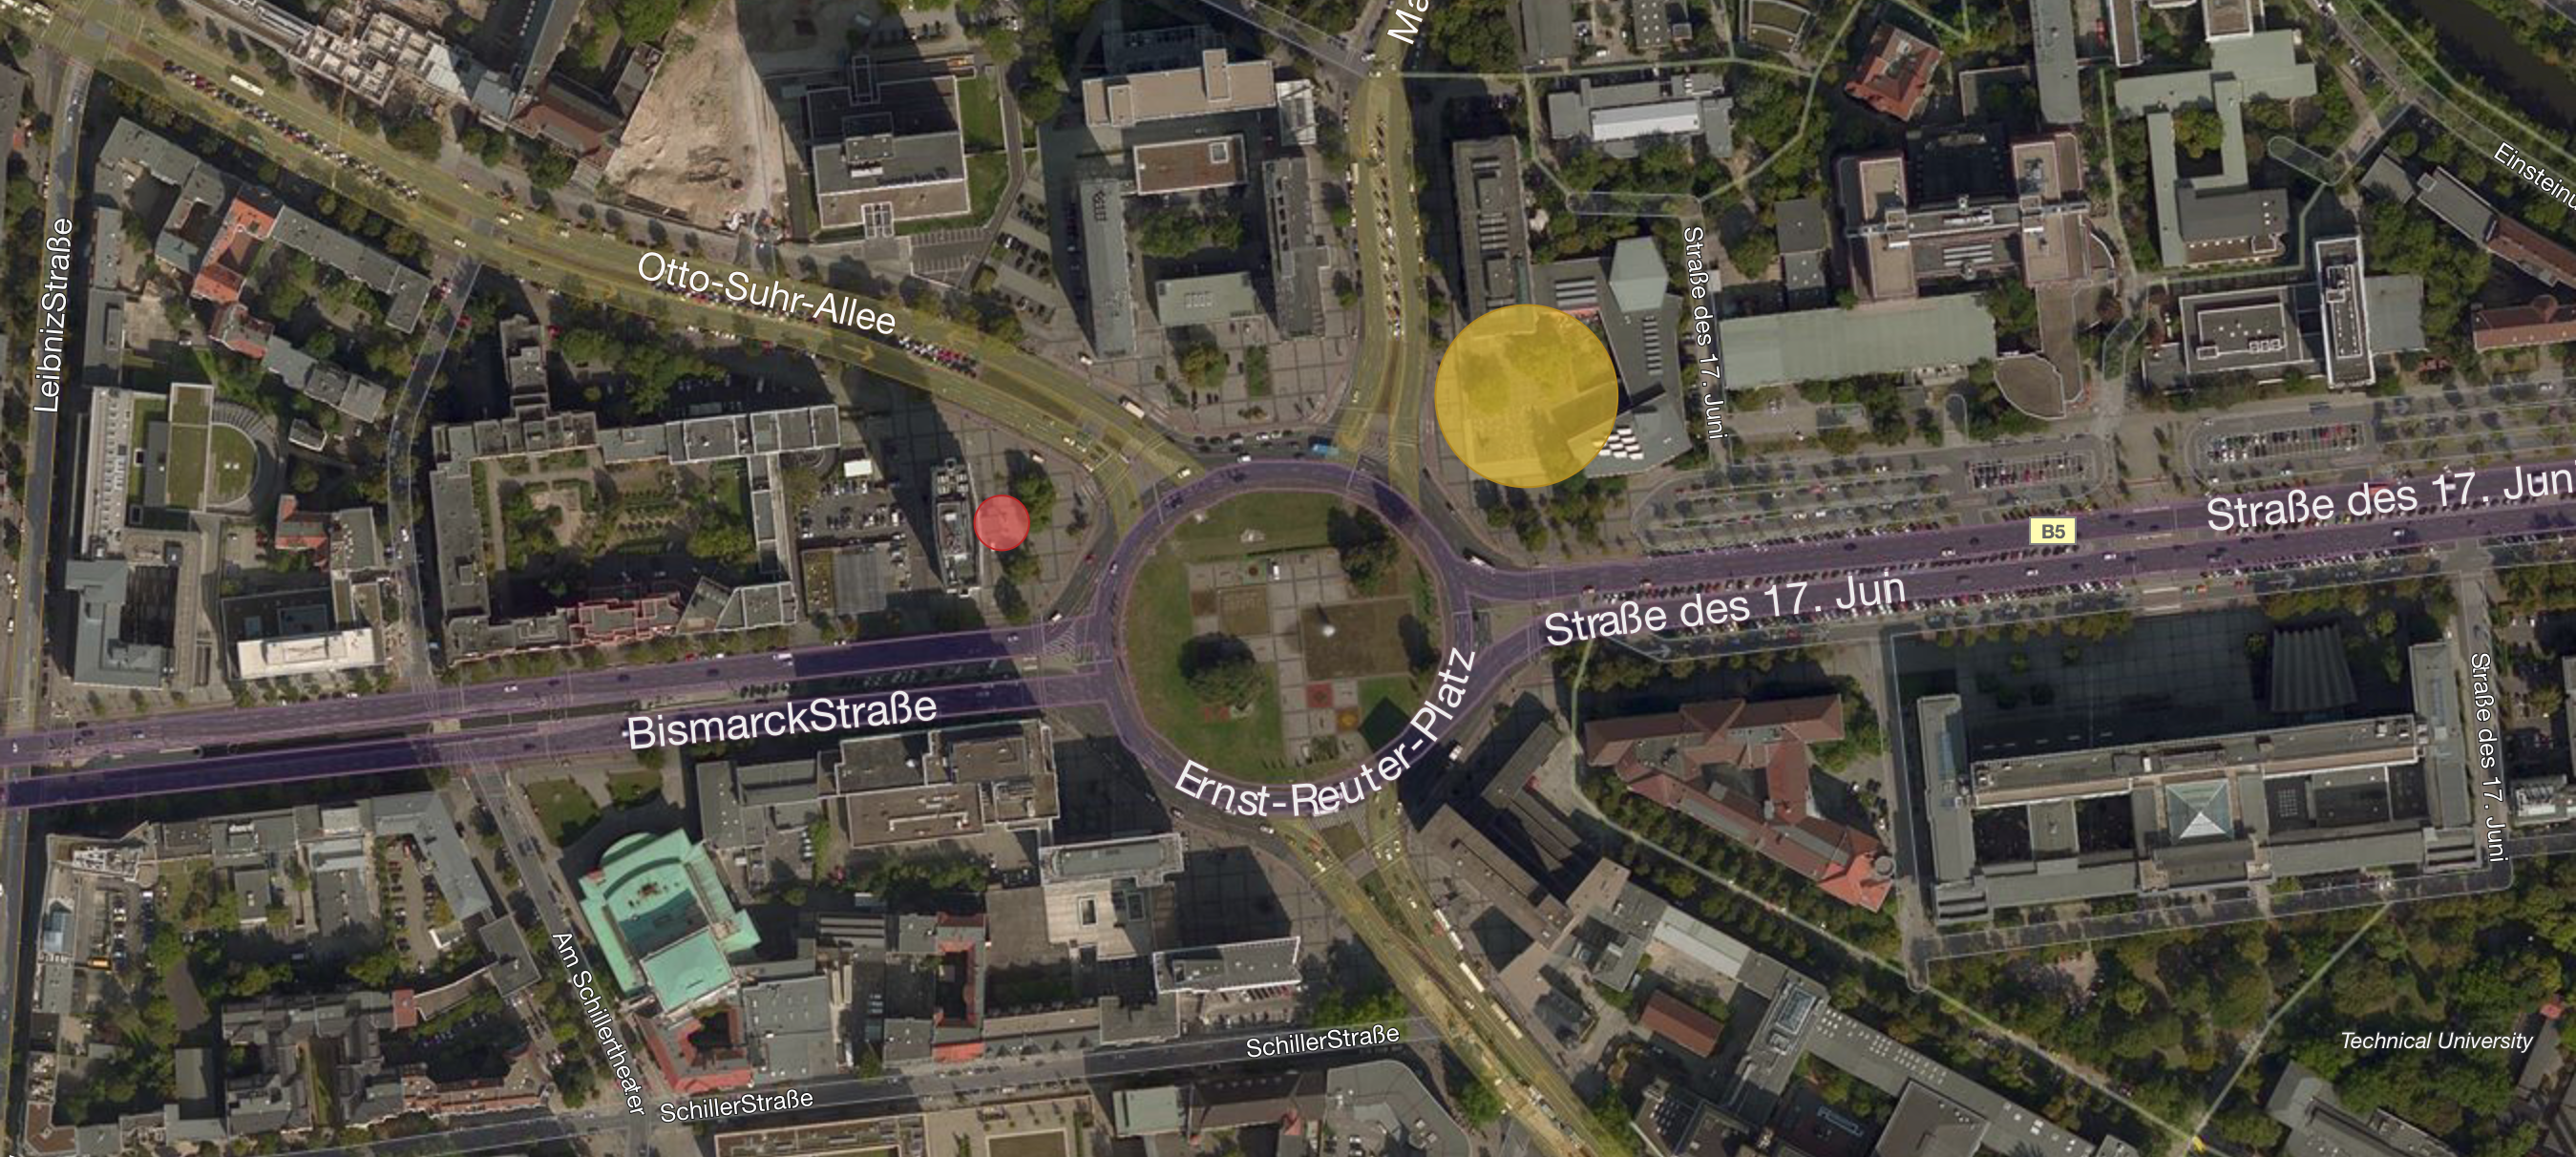
\includegraphics{images/pedestrians_map_satelite.png}
\caption{map\_overview}
\end{figure}

    \begin{Verbatim}[commandchars=\\\{\}]
{\color{incolor}In [{\color{incolor}17}]:} \PY{n}{times} \PY{o}{=} \PY{n}{pd}\PY{o}{.}\PY{n}{DatetimeIndex}\PY{p}{(}\PY{n}{df\PYZus{}pedestrians}\PY{o}{.}\PY{n}{Timestamp}\PY{p}{)}
         \PY{n}{grouped} \PY{o}{=} \PY{n}{df\PYZus{}pedestrians}\PY{o}{.}\PY{n}{groupby}\PY{p}{(}\PY{p}{[}\PY{n}{times}\PY{o}{.}\PY{n}{hour}\PY{p}{]}\PY{p}{)}
         \PY{n}{grouped\PYZus{}direction\PYZus{}count} \PY{o}{=} \PY{n}{grouped}\PY{p}{[}\PY{l+s+s1}{\PYZsq{}}\PY{l+s+s1}{Direction}\PY{l+s+s1}{\PYZsq{}}\PY{p}{]}\PY{o}{.}\PY{n}{count}\PY{p}{(}\PY{p}{)}
         
         \PY{n}{hist\PYZus{}in\PYZus{}out\PYZus{}pedestrians} \PY{o}{=} \PY{n}{sns}\PY{o}{.}\PY{n}{barplot}\PY{p}{(}\PY{n}{x}\PY{o}{=}\PY{n}{grouped\PYZus{}direction\PYZus{}count}\PY{o}{.}\PY{n}{index}\PY{p}{,} \PY{n}{y}\PY{o}{=}\PY{n}{grouped\PYZus{}direction\PYZus{}count}\PY{o}{.}\PY{n}{values}\PY{p}{)}
         \PY{n}{hist\PYZus{}in\PYZus{}out\PYZus{}pedestrians}\PY{o}{.}\PY{n}{set}\PY{p}{(}\PY{n}{xlabel}\PY{o}{=}\PY{l+s+s1}{\PYZsq{}}\PY{l+s+s1}{Hour}\PY{l+s+s1}{\PYZsq{}}\PY{p}{,} \PY{n}{ylabel}\PY{o}{=}\PY{l+s+s1}{\PYZsq{}}\PY{l+s+s1}{Pedestrians passed}\PY{l+s+s1}{\PYZsq{}}\PY{p}{)}
         
         \PY{n}{sns}\PY{o}{.}\PY{n}{distplot}
         \PY{n}{plt}\PY{o}{.}\PY{n}{gca}\PY{p}{(}\PY{p}{)}\PY{o}{.}\PY{n}{spines}\PY{p}{[}\PY{l+s+s1}{\PYZsq{}}\PY{l+s+s1}{right}\PY{l+s+s1}{\PYZsq{}}\PY{p}{]}\PY{o}{.}\PY{n}{set\PYZus{}visible}\PY{p}{(}\PY{k+kc}{False}\PY{p}{)}
         \PY{n}{plt}\PY{o}{.}\PY{n}{gca}\PY{p}{(}\PY{p}{)}\PY{o}{.}\PY{n}{spines}\PY{p}{[}\PY{l+s+s1}{\PYZsq{}}\PY{l+s+s1}{top}\PY{l+s+s1}{\PYZsq{}}\PY{p}{]}\PY{o}{.}\PY{n}{set\PYZus{}visible}\PY{p}{(}\PY{k+kc}{False}\PY{p}{)}
         \PY{n}{plt}\PY{o}{.}\PY{n}{show}\PY{p}{(}\PY{p}{)}
\end{Verbatim}


    \begin{center}
    \adjustimage{max size={0.9\linewidth}{0.9\paperheight}}{output_46_0.png}
    \end{center}
    { \hspace*{\fill} \\}
    
    \begin{figure}
\centering
\includegraphics{images/pedestrian_count_avg_hourly.png}
\caption{map\_overview}
\end{figure}

    \begin{Verbatim}[commandchars=\\\{\}]
{\color{incolor}In [{\color{incolor}18}]:} \PY{c+c1}{\PYZsh{} as bar chart}
         \PY{n}{bar\PYZus{}width} \PY{o}{=} \PY{l+m+mf}{0.3}
         \PY{n}{bars1} \PY{o}{=} \PY{p}{[}\PY{n}{count\PYZus{}walked\PYZus{}IN\PYZus{}af}\PY{p}{,} \PY{n}{count\PYZus{}walked\PYZus{}IN\PYZus{}tel}\PY{p}{]}
         \PY{n}{bars2} \PY{o}{=} \PY{p}{[}\PY{n}{count\PYZus{}walked\PYZus{}OUT\PYZus{}af}\PY{p}{,} \PY{n}{count\PYZus{}walked\PYZus{}OUT\PYZus{}tel}\PY{p}{]}
         \PY{c+c1}{\PYZsh{} x position of bars}
         \PY{n}{r1} \PY{o}{=} \PY{n}{np}\PY{o}{.}\PY{n}{arange}\PY{p}{(}\PY{n+nb}{len}\PY{p}{(}\PY{n}{bars1}\PY{p}{)}\PY{p}{)}
         \PY{n}{r2} \PY{o}{=} \PY{p}{[}\PY{n}{x} \PY{o}{+} \PY{n}{bar\PYZus{}width} \PY{k}{for} \PY{n}{x} \PY{o+ow}{in} \PY{n}{r1}\PY{p}{]}
         \PY{c+c1}{\PYZsh{} create bars1}
         \PY{n}{plt}\PY{o}{.}\PY{n}{bar}\PY{p}{(}\PY{n}{r1}\PY{p}{,} \PY{n}{bars1}\PY{p}{,} \PY{n}{width}\PY{o}{=}\PY{n}{bar\PYZus{}width}\PY{p}{,} \PY{n}{color}\PY{o}{=}\PY{p}{(}\PY{l+m+mf}{0.3}\PY{p}{,}\PY{l+m+mf}{0.1}\PY{p}{,}\PY{l+m+mf}{0.4}\PY{p}{,}\PY{l+m+mf}{0.6}\PY{p}{)}\PY{p}{,} \PY{n}{capsize}\PY{o}{=}\PY{l+m+mi}{7}\PY{p}{,} \PY{n}{label}\PY{o}{=}\PY{l+s+s1}{\PYZsq{}}\PY{l+s+s1}{IN}\PY{l+s+s1}{\PYZsq{}}\PY{p}{)}
         \PY{n}{plt}\PY{o}{.}\PY{n}{bar}\PY{p}{(}\PY{n}{r2}\PY{p}{,} \PY{n}{bars2}\PY{p}{,} \PY{n}{width}\PY{o}{=}\PY{n}{bar\PYZus{}width}\PY{p}{,} \PY{n}{color}\PY{o}{=}\PY{p}{(}\PY{l+m+mf}{0.3}\PY{p}{,}\PY{l+m+mf}{0.5}\PY{p}{,}\PY{l+m+mf}{0.4}\PY{p}{,}\PY{l+m+mf}{0.6}\PY{p}{)}\PY{p}{,} \PY{n}{capsize}\PY{o}{=}\PY{l+m+mi}{7}\PY{p}{,} \PY{n}{label}\PY{o}{=}\PY{l+s+s1}{\PYZsq{}}\PY{l+s+s1}{OUT}\PY{l+s+s1}{\PYZsq{}}\PY{p}{)}
         
         \PY{c+c1}{\PYZsh{} general layout}
         \PY{n}{plt}\PY{o}{.}\PY{n}{xticks}\PY{p}{(}\PY{p}{[}\PY{l+m+mf}{0.15}\PY{p}{,} \PY{l+m+mf}{1.15}\PY{p}{]}\PY{p}{,} \PY{p}{[}\PY{l+s+s1}{\PYZsq{}}\PY{l+s+s1}{AF}\PY{l+s+s1}{\PYZsq{}}\PY{p}{,} \PY{l+s+s1}{\PYZsq{}}\PY{l+s+s1}{Telekom}\PY{l+s+s1}{\PYZsq{}}\PY{p}{]}\PY{p}{)}
         \PY{n}{plt}\PY{o}{.}\PY{n}{ylabel}\PY{p}{(}\PY{l+s+s1}{\PYZsq{}}\PY{l+s+s1}{Pedestrians Throughput}\PY{l+s+s1}{\PYZsq{}}\PY{p}{)}
         \PY{n}{plt}\PY{o}{.}\PY{n}{gca}\PY{p}{(}\PY{p}{)}\PY{o}{.}\PY{n}{yaxis}\PY{o}{.}\PY{n}{set\PYZus{}label\PYZus{}position}\PY{p}{(}\PY{l+s+s2}{\PYZdq{}}\PY{l+s+s2}{right}\PY{l+s+s2}{\PYZdq{}}\PY{p}{)}
         \PY{n}{plt}\PY{o}{.}\PY{n}{locator\PYZus{}params}\PY{p}{(}\PY{n}{axis}\PY{o}{=}\PY{l+s+s1}{\PYZsq{}}\PY{l+s+s1}{y}\PY{l+s+s1}{\PYZsq{}}\PY{p}{,} \PY{n}{nbins}\PY{o}{=}\PY{l+m+mi}{5}\PY{p}{)}
         \PY{n}{plt}\PY{o}{.}\PY{n}{legend}\PY{p}{(}\PY{p}{)}
         \PY{n}{plt}\PY{o}{.}\PY{n}{tick\PYZus{}params}\PY{p}{(}\PY{n}{top}\PY{o}{=}\PY{k+kc}{False}\PY{p}{,} \PY{n}{bottom}\PY{o}{=}\PY{k+kc}{True}\PY{p}{,} \PY{n}{left}\PY{o}{=}\PY{k+kc}{False}\PY{p}{,} \PY{n}{right}\PY{o}{=}\PY{k+kc}{False}\PY{p}{,} \PY{n}{labelleft}\PY{o}{=}\PY{k+kc}{True}\PY{p}{,} \PY{n}{labelbottom}\PY{o}{=}\PY{k+kc}{True}\PY{p}{)}
         \PY{c+c1}{\PYZsh{} Hide the right and top spines}
         \PY{n}{plt}\PY{o}{.}\PY{n}{gca}\PY{p}{(}\PY{p}{)}\PY{o}{.}\PY{n}{spines}\PY{p}{[}\PY{l+s+s1}{\PYZsq{}}\PY{l+s+s1}{right}\PY{l+s+s1}{\PYZsq{}}\PY{p}{]}\PY{o}{.}\PY{n}{set\PYZus{}visible}\PY{p}{(}\PY{k+kc}{False}\PY{p}{)}
         \PY{n}{plt}\PY{o}{.}\PY{n}{gca}\PY{p}{(}\PY{p}{)}\PY{o}{.}\PY{n}{spines}\PY{p}{[}\PY{l+s+s1}{\PYZsq{}}\PY{l+s+s1}{top}\PY{l+s+s1}{\PYZsq{}}\PY{p}{]}\PY{o}{.}\PY{n}{set\PYZus{}visible}\PY{p}{(}\PY{k+kc}{False}\PY{p}{)}
         
         \PY{c+c1}{\PYZsh{} Show graphic}
         \PY{n}{plt}\PY{o}{.}\PY{n}{show}\PY{p}{(}\PY{p}{)}
\end{Verbatim}


    \begin{center}
    \adjustimage{max size={0.9\linewidth}{0.9\paperheight}}{output_48_0.png}
    \end{center}
    { \hspace*{\fill} \\}
    
    \begin{Verbatim}[commandchars=\\\{\}]
{\color{incolor}In [{\color{incolor}19}]:} \PY{n+nb}{print}\PY{p}{(}\PY{l+s+s1}{\PYZsq{}}\PY{l+s+s1}{The buildings must be spawning pedestrians from the cellar 😱🧙}\PY{l+s+s1}{\PYZsq{}}\PY{p}{)}
         \PY{n+nb}{print}\PY{p}{(}\PY{l+s+s1}{\PYZsq{}}\PY{l+s+s1}{Or there might be different entries to the building...}\PY{l+s+s1}{\PYZsq{}}\PY{p}{)}
\end{Verbatim}


    \begin{Verbatim}[commandchars=\\\{\}]
The buildings must be spawning pedestrians from the cellar 😱🧙
Or there might be different entries to the building{\ldots}

    \end{Verbatim}

    \begin{figure}
\centering
\includegraphics{images/pedestrains_average_count_by_day.png}
\caption{pedestrians\_average\_per\_day}
\end{figure}

    \subsection{WIFI Connections}\label{wifi-connections}

\begin{figure}
\centering
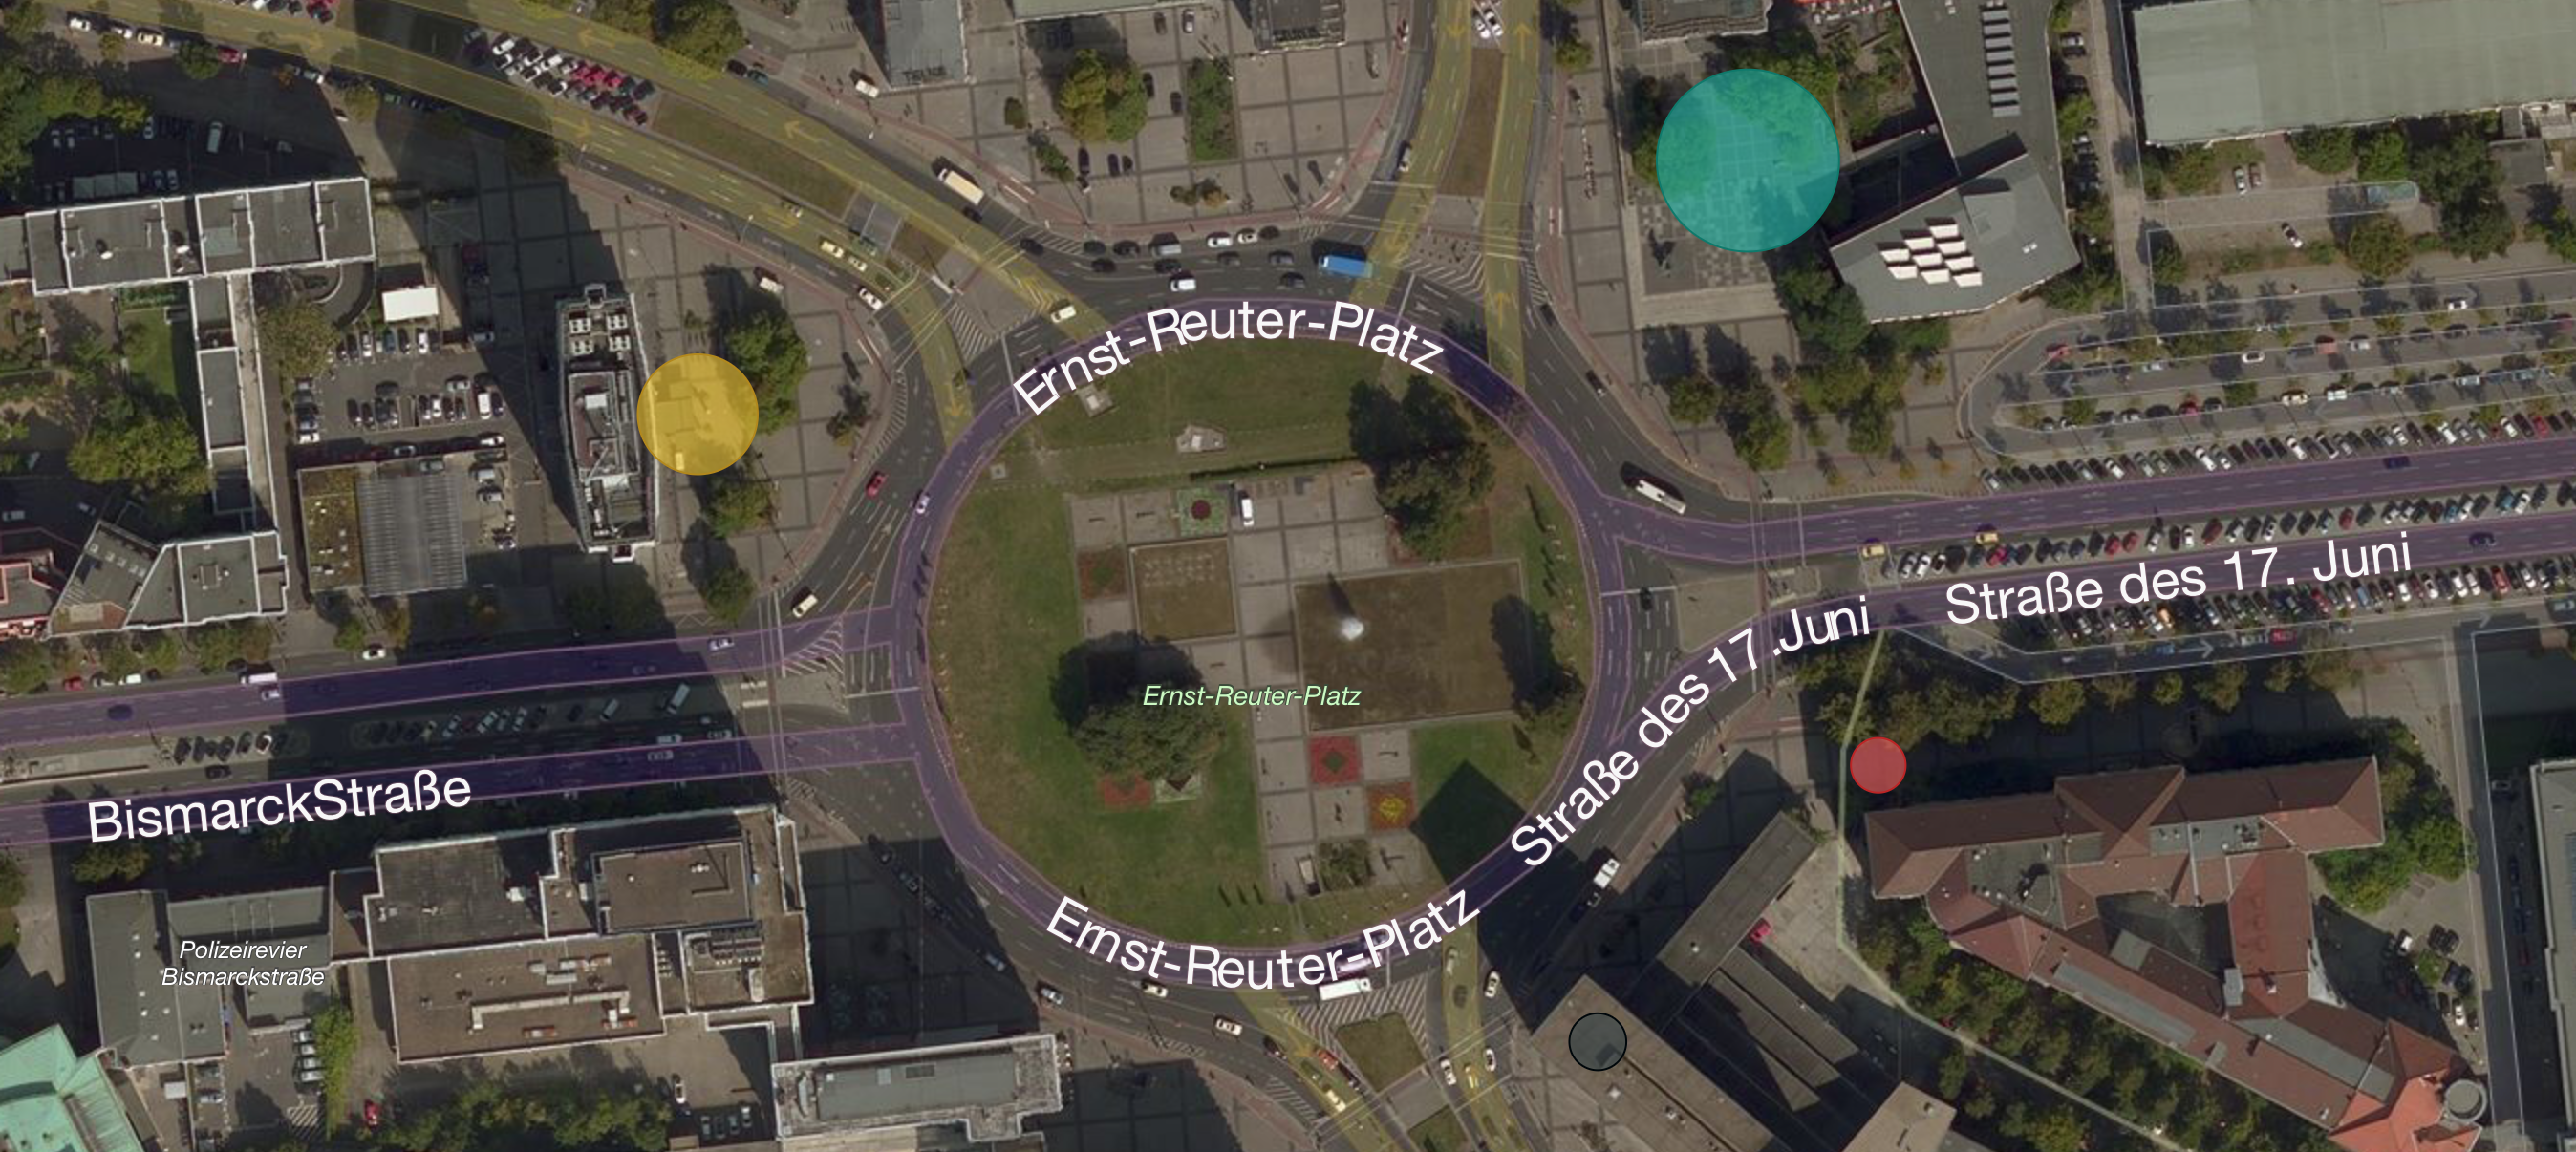
\includegraphics{images/wifi_map_satelite.png}
\caption{map\_overview}
\end{figure}

    \begin{Verbatim}[commandchars=\\\{\}]
{\color{incolor}In [{\color{incolor}20}]:} \PY{n}{df\PYZus{}wifi\PYZus{}original} \PY{o}{=} \PY{n}{pd}\PY{o}{.}\PY{n}{read\PYZus{}csv}\PY{p}{(}\PY{l+s+s1}{\PYZsq{}}\PY{l+s+s1}{data/wifi.csv}\PY{l+s+s1}{\PYZsq{}}\PY{p}{,} \PY{n}{sep}\PY{o}{=}\PY{l+s+s2}{\PYZdq{}}\PY{l+s+s2}{ }\PY{l+s+s2}{\PYZdq{}}\PY{p}{)}
         \PY{n}{df\PYZus{}wifi} \PY{o}{=} \PY{n}{df\PYZus{}wifi\PYZus{}original}
         \PY{n}{df\PYZus{}wifi}\PY{p}{[}\PY{l+s+s1}{\PYZsq{}}\PY{l+s+s1}{Timestamp}\PY{l+s+s1}{\PYZsq{}}\PY{p}{]} \PY{o}{=} \PY{n}{pd}\PY{o}{.}\PY{n}{to\PYZus{}datetime}\PY{p}{(}\PY{n}{df\PYZus{}wifi}\PY{p}{[}\PY{l+s+s1}{\PYZsq{}}\PY{l+s+s1}{Timestamp}\PY{l+s+s1}{\PYZsq{}}\PY{p}{]}\PY{o}{.}\PY{n}{astype}\PY{p}{(}\PY{n+nb}{int}\PY{p}{)}\PY{p}{,} \PY{n}{unit}\PY{o}{=}\PY{l+s+s1}{\PYZsq{}}\PY{l+s+s1}{ms}\PY{l+s+s1}{\PYZsq{}}\PY{p}{)}
         
         \PY{n}{wifi\PYZus{}times} \PY{o}{=} \PY{n}{df\PYZus{}wifi}\PY{p}{[}\PY{l+s+s1}{\PYZsq{}}\PY{l+s+s1}{Timestamp}\PY{l+s+s1}{\PYZsq{}}\PY{p}{]}
         \PY{n}{wifi\PYZus{}grouped\PYZus{}sum} \PY{o}{=} \PY{n}{df\PYZus{}wifi}\PY{o}{.}\PY{n}{groupby}\PY{p}{(}\PY{p}{[}\PY{n}{wifi\PYZus{}times}\PY{o}{.}\PY{n}{dt}\PY{o}{.}\PY{n}{hour}\PY{p}{]}\PY{p}{)}\PY{o}{.}\PY{n}{sum}\PY{p}{(}\PY{p}{)}
         \PY{n}{np}\PY{o}{.}\PY{n}{random}\PY{o}{.}\PY{n}{seed}\PY{p}{(}\PY{l+m+mi}{19680801}\PY{p}{)}
         \PY{n}{x} \PY{o}{=} \PY{n}{wifi\PYZus{}grouped\PYZus{}sum}\PY{o}{.}\PY{n}{index}
         \PY{n}{y} \PY{o}{=} \PY{n}{wifi\PYZus{}grouped\PYZus{}sum}\PY{p}{[}\PY{l+s+s1}{\PYZsq{}}\PY{l+s+s1}{DevicesTracked}\PY{l+s+s1}{\PYZsq{}}\PY{p}{]}
         \PY{n}{bubble\PYZus{}area} \PY{o}{=} \PY{p}{(}\PY{n}{wifi\PYZus{}grouped\PYZus{}sum}\PY{p}{[}\PY{l+s+s1}{\PYZsq{}}\PY{l+s+s1}{ApproxVerweildauerSek}\PY{l+s+s1}{\PYZsq{}}\PY{p}{]} \PY{o}{/} \PY{l+m+mi}{60}\PY{p}{)}
         \PY{n}{colors} \PY{o}{=} \PY{n}{np}\PY{o}{.}\PY{n}{random}\PY{o}{.}\PY{n}{rand}\PY{p}{(}\PY{l+m+mi}{24}\PY{p}{)}
         
         \PY{n}{wifi\PYZus{}scatter} \PY{o}{=} \PY{n}{plt}\PY{o}{.}\PY{n}{scatter}\PY{p}{(}\PY{n}{x}\PY{p}{,} \PY{n}{y}\PY{p}{,} \PY{n}{s}\PY{o}{=}\PY{n}{bubble\PYZus{}area}\PY{p}{,} \PY{n}{c}\PY{o}{=}\PY{n}{colors}\PY{p}{,} \PY{n}{alpha}\PY{o}{=}\PY{l+m+mf}{0.5}\PY{p}{)}
         \PY{c+c1}{\PYZsh{} general layout}
         \PY{n}{plt}\PY{o}{.}\PY{n}{xlabel}\PY{p}{(}\PY{l+s+s1}{\PYZsq{}}\PY{l+s+s1}{Hour of the Day}\PY{l+s+s1}{\PYZsq{}}\PY{p}{)}
         \PY{n}{plt}\PY{o}{.}\PY{n}{tick\PYZus{}params}\PY{p}{(}\PY{n}{top}\PY{o}{=}\PY{k+kc}{False}\PY{p}{,} \PY{n}{bottom}\PY{o}{=}\PY{k+kc}{False}\PY{p}{,} \PY{n}{left}\PY{o}{=}\PY{k+kc}{False}\PY{p}{,} \PY{n}{right}\PY{o}{=}\PY{k+kc}{False}\PY{p}{,} \PY{n}{labelleft}\PY{o}{=}\PY{k+kc}{True}\PY{p}{,} \PY{n}{labelbottom}\PY{o}{=}\PY{k+kc}{True}\PY{p}{)}
         \PY{c+c1}{\PYZsh{} Hide the right and top spines}
         \PY{n}{plt}\PY{o}{.}\PY{n}{gca}\PY{p}{(}\PY{p}{)}\PY{o}{.}\PY{n}{spines}\PY{p}{[}\PY{l+s+s1}{\PYZsq{}}\PY{l+s+s1}{right}\PY{l+s+s1}{\PYZsq{}}\PY{p}{]}\PY{o}{.}\PY{n}{set\PYZus{}visible}\PY{p}{(}\PY{k+kc}{False}\PY{p}{)}
         \PY{n}{plt}\PY{o}{.}\PY{n}{gca}\PY{p}{(}\PY{p}{)}\PY{o}{.}\PY{n}{spines}\PY{p}{[}\PY{l+s+s1}{\PYZsq{}}\PY{l+s+s1}{left}\PY{l+s+s1}{\PYZsq{}}\PY{p}{]}\PY{o}{.}\PY{n}{set\PYZus{}visible}\PY{p}{(}\PY{k+kc}{False}\PY{p}{)}
         \PY{n}{plt}\PY{o}{.}\PY{n}{gca}\PY{p}{(}\PY{p}{)}\PY{o}{.}\PY{n}{spines}\PY{p}{[}\PY{l+s+s1}{\PYZsq{}}\PY{l+s+s1}{top}\PY{l+s+s1}{\PYZsq{}}\PY{p}{]}\PY{o}{.}\PY{n}{set\PYZus{}visible}\PY{p}{(}\PY{k+kc}{False}\PY{p}{)}
         \PY{n}{plt}\PY{o}{.}\PY{n}{gca}\PY{p}{(}\PY{p}{)}\PY{o}{.}\PY{n}{spines}\PY{p}{[}\PY{l+s+s1}{\PYZsq{}}\PY{l+s+s1}{bottom}\PY{l+s+s1}{\PYZsq{}}\PY{p}{]}\PY{o}{.}\PY{n}{set\PYZus{}visible}\PY{p}{(}\PY{k+kc}{False}\PY{p}{)}
         \PY{c+c1}{\PYZsh{} put some text for y\PYZhy{}label}
         \PY{n}{plt}\PY{o}{.}\PY{n}{text}\PY{p}{(}\PY{l+m+mf}{0.05}\PY{p}{,}\PY{l+m+mf}{0.95}\PY{p}{,} \PY{l+s+s1}{\PYZsq{}}\PY{l+s+s1}{Devices Tracked}\PY{l+s+s1}{\PYZsq{}}\PY{p}{,} \PY{n}{fontsize}\PY{o}{=}\PY{l+s+s2}{\PYZdq{}}\PY{l+s+s2}{15}\PY{l+s+s2}{\PYZdq{}}\PY{p}{,} \PY{n}{ha}\PY{o}{=}\PY{l+s+s2}{\PYZdq{}}\PY{l+s+s2}{right}\PY{l+s+s2}{\PYZdq{}}\PY{p}{,} \PY{n}{va}\PY{o}{=}\PY{l+s+s2}{\PYZdq{}}\PY{l+s+s2}{top}\PY{l+s+s2}{\PYZdq{}}\PY{p}{,} \PY{n}{transform}\PY{o}{=}\PY{n}{plt}\PY{o}{.}\PY{n}{gca}\PY{p}{(}\PY{p}{)}\PY{o}{.}\PY{n}{transAxes}\PY{p}{)}
         \PY{c+c1}{\PYZsh{} supress pyplot output}
         \PY{n}{\PYZus{}} \PY{o}{=} \PY{n}{plt}\PY{o}{.}\PY{n}{show}
\end{Verbatim}


    \begin{center}
    \adjustimage{max size={0.9\linewidth}{0.9\paperheight}}{output_52_0.png}
    \end{center}
    { \hspace*{\fill} \\}
    
    \begin{Verbatim}[commandchars=\\\{\}]
{\color{incolor}In [{\color{incolor}21}]:} \PY{n+nb}{print}\PY{p}{(}\PY{l+s+s1}{\PYZsq{}}\PY{l+s+s1}{Median der Verweildauer in Stunden: }\PY{l+s+s1}{\PYZsq{}} \PY{o}{+} \PY{n+nb}{str}\PY{p}{(}\PY{n+nb}{round}\PY{p}{(}\PY{n}{wifi\PYZus{}grouped\PYZus{}sum}\PY{p}{[}\PY{l+s+s1}{\PYZsq{}}\PY{l+s+s1}{ApproxVerweildauerSek}\PY{l+s+s1}{\PYZsq{}}\PY{p}{]}\PY{o}{.}\PY{n}{median}\PY{p}{(}\PY{p}{)} \PY{o}{/} \PY{l+m+mi}{60} \PY{o}{/} \PY{l+m+mi}{60}\PY{p}{,} \PY{l+m+mi}{2}\PY{p}{)}\PY{p}{)}\PY{p}{)}
         \PY{n+nb}{print}\PY{p}{(}\PY{l+s+s1}{\PYZsq{}}\PY{l+s+s1}{Verweildauer zwischen 2:00 und 2:59 Uhr in Stunden: }\PY{l+s+s1}{\PYZsq{}} \PY{o}{+} \PY{n+nb}{str}\PY{p}{(}\PY{n+nb}{round}\PY{p}{(}\PY{n}{wifi\PYZus{}grouped\PYZus{}sum}\PY{o}{.}\PY{n}{loc}\PY{p}{[}\PY{l+m+mi}{2}\PY{p}{,} \PY{l+s+s1}{\PYZsq{}}\PY{l+s+s1}{ApproxVerweildauerSek}\PY{l+s+s1}{\PYZsq{}}\PY{p}{]} \PY{o}{/} \PY{l+m+mi}{60} \PY{o}{/} \PY{l+m+mi}{60}\PY{p}{)}\PY{p}{)} \PY{o}{+} \PY{l+s+s1}{\PYZsq{}}\PY{l+s+s1}{ 😯}\PY{l+s+s1}{\PYZsq{}}\PY{p}{)}
\end{Verbatim}


    \begin{Verbatim}[commandchars=\\\{\}]
Median der Verweildauer in Stunden: 6.02
Verweildauer zwischen 2:00 und 2:59 Uhr in Stunden: 32.0 😯

    \end{Verbatim}

    \begin{figure}
\centering
\includegraphics{images/wifi_connection_average_per_day.png}
\caption{map\_overview}
\end{figure}

    \begin{figure}
\centering
\includegraphics{images/wifi_connection_density.png}
\caption{map\_overview}
\end{figure}

    \begin{figure}
\centering
\includegraphics{images/doener.jpg}
\caption{map\_overview}
\end{figure}

    \begin{figure}
\centering
\includegraphics{images/doener_alt.png}
\caption{doener\_alt}
\end{figure}

    \begin{Verbatim}[commandchars=\\\{\}]
{\color{incolor}In [{\color{incolor}22}]:} \PY{c+c1}{\PYZsh{}\PYZsh{} TODO: take center of ernst\PYZhy{}reuter platz as location=POINT}
         \PY{n+nb}{map} \PY{o}{=} \PY{n}{folium}\PY{o}{.}\PY{n}{Map}\PY{p}{(}\PY{n}{location}\PY{o}{=}\PY{n}{ernst\PYZus{}reuter\PYZus{}platz\PYZus{}center}\PY{p}{,} \PY{n}{zoom\PYZus{}start}\PY{o}{=}\PY{l+m+mi}{17}\PY{p}{)}
         
         
         \PY{k}{for} \PY{n}{key} \PY{o+ow}{in} \PY{n}{wifi\PYZus{}latlon}\PY{p}{:}
             \PY{n}{folium}\PY{o}{.}\PY{n}{Circle}\PY{p}{(}
                 \PY{n}{radius}\PY{o}{=}\PY{l+m+mi}{50}\PY{p}{,}
                 \PY{n}{location}\PY{o}{=}\PY{n}{wifi\PYZus{}latlon}\PY{p}{[}\PY{n}{key}\PY{p}{]}\PY{p}{,}
                 \PY{n}{popup}\PY{o}{=}\PY{n}{key}\PY{p}{,}
                 \PY{n}{color}\PY{o}{=}\PY{l+s+s1}{\PYZsq{}}\PY{l+s+s1}{\PYZsh{}3186cc}\PY{l+s+s1}{\PYZsq{}}\PY{p}{,}
                 \PY{n}{fill}\PY{o}{=}\PY{k+kc}{True}
             \PY{p}{)}\PY{o}{.}\PY{n}{add\PYZus{}to}\PY{p}{(}\PY{n+nb}{map}\PY{p}{)}
             
         \PY{k}{for} \PY{n}{key} \PY{o+ow}{in} \PY{n}{pedestrian\PYZus{}latlon}\PY{p}{:}
             \PY{n}{folium}\PY{o}{.}\PY{n}{Marker}\PY{p}{(}
                 \PY{n}{location}\PY{o}{=}\PY{n}{pedestrian\PYZus{}latlon}\PY{p}{[}\PY{n}{key}\PY{p}{]}\PY{p}{,}
                 \PY{n}{popup}\PY{o}{=}\PY{n}{key}\PY{p}{,}
                 \PY{n}{icon}\PY{o}{=}\PY{n}{folium}\PY{o}{.}\PY{n}{Icon}\PY{p}{(}\PY{n}{icon}\PY{o}{=}\PY{l+s+s1}{\PYZsq{}}\PY{l+s+s1}{info\PYZhy{}sign}\PY{l+s+s1}{\PYZsq{}}\PY{p}{)}
             \PY{p}{)}\PY{o}{.}\PY{n}{add\PYZus{}to}\PY{p}{(}\PY{n+nb}{map}\PY{p}{)}
             
         \PY{k}{for} \PY{n}{key} \PY{o+ow}{in} \PY{n}{traffic\PYZus{}latlon}\PY{p}{:}
             \PY{n}{folium}\PY{o}{.}\PY{n}{Marker}\PY{p}{(}
                 \PY{n}{location}\PY{o}{=}\PY{n}{traffic\PYZus{}latlon}\PY{p}{[}\PY{n}{key}\PY{p}{]}\PY{p}{,}
                 \PY{n}{popup}\PY{o}{=}\PY{n}{key}\PY{p}{,}
                 \PY{n}{icon}\PY{o}{=}\PY{n}{folium}\PY{o}{.}\PY{n}{Icon}\PY{p}{(}\PY{n}{color}\PY{o}{=}\PY{l+s+s1}{\PYZsq{}}\PY{l+s+s1}{red}\PY{l+s+s1}{\PYZsq{}}\PY{p}{,}\PY{n}{icon}\PY{o}{=}\PY{l+s+s1}{\PYZsq{}}\PY{l+s+s1}{info\PYZhy{}sign}\PY{l+s+s1}{\PYZsq{}}\PY{p}{)}
             \PY{p}{)}\PY{o}{.}\PY{n}{add\PYZus{}to}\PY{p}{(}\PY{n+nb}{map}\PY{p}{)}
         
         \PY{k}{for} \PY{n}{key} \PY{o+ow}{in} \PY{n}{parking\PYZus{}latlon}\PY{p}{:}
             \PY{n}{folium}\PY{o}{.}\PY{n}{Circle}\PY{p}{(}
                 \PY{n}{radius}\PY{o}{=}\PY{l+m+mi}{2}\PY{p}{,}
                 \PY{n}{location}\PY{o}{=}\PY{n}{parking\PYZus{}latlon}\PY{p}{[}\PY{n}{key}\PY{p}{]}\PY{p}{,}
                 \PY{n}{popup}\PY{o}{=}\PY{n}{key}\PY{p}{,}
                 \PY{n}{color}\PY{o}{=}\PY{l+s+s1}{\PYZsq{}}\PY{l+s+s1}{red}\PY{l+s+s1}{\PYZsq{}}\PY{p}{,}
                 \PY{n}{fill}\PY{o}{=}\PY{k+kc}{True}
             \PY{p}{)}\PY{o}{.}\PY{n}{add\PYZus{}to}\PY{p}{(}\PY{n+nb}{map}\PY{p}{)}
         
         \PY{n+nb}{map}
\end{Verbatim}


\begin{Verbatim}[commandchars=\\\{\}]
{\color{outcolor}Out[{\color{outcolor}22}]:} <folium.folium.Map at 0x1a157b8d68>
\end{Verbatim}
            

    % Add a bibliography block to the postdoc
    
    
    
    \end{document}
